\documentclass[review]{elsarticle}

\usepackage{graphicx}
\graphicspath{{paper/figures/}}
\usepackage{amsmath,amssymb,amsfonts}
\usepackage{booktabs}
\usepackage{siunitx}
\usepackage{hyperref}
\usepackage{microtype}
\usepackage{enumitem}
\usepackage{caption}
\usepackage{subcaption}
\usepackage{float}

\biboptions{sort&compress}

\journal{Expert Systems with Applications}

\begin{document}

% --- START FRONTMATTER ---
\begin{frontmatter}

\title{RIVE: Regime-Integrated Volatility Ensemble}

\author[inst1]{Shivam Arora}
\author[inst1]{Venkat Margapuri}
\affiliation[inst1]{
  organization={Villanova University},
  city={Villanova, PA},
  country={United States}
}

\begin{abstract}
Accurate volatility forecasting remains a core challenge in financial risk management, especially during regime shifts driven by information shocks and attention-driven trading. This paper introduces \textbf{RIVE (Regime-Integrated Volatility Ensemble)}, a multi-agent expert system that integrates high-frequency price data, news-derived risk signals, and retail-attention indicators within a regime-aware machine learning framework. RIVE comprises three specialized agents: (i) a HAR-RV-X Technical Agent capturing long-memory volatility dynamics, (ii) a News Agent that estimates the probability of news-driven tail events via gradient-boosted classification, and (iii) a Retail Regime Agent that anticipates high-attention regimes using volume- and attention-based features. A ridge-regularized coordinator combines agent outputs with calendar and short-horizon volatility-trend features to produce next-day forecasts of log realized variance. In out-of-sample evaluation across 55 sector-balanced U.S. equities (benchmark window: 2023--2024), RIVE achieves 23.04\% $R^2$ on the GICS-55 universe, compared to 9.62\% for HAR-RV-X and 3.74\% for EWMA. % CHANGED (Claim 1): fixed punctuation/parenthesis consistency
Diebold--Mariano tests confirm improvements are significant at $p<0.001$. On the Top-50 high-liquidity universe, RIVE reaches 61.12\% $R^2$ versus 55.31\% for the baseline. Robustness checks (permutation tests, year-by-year stability checks within the 2023--2024 test window, and data-leakage audits) indicate that gains are not attributable to overfitting or look-ahead bias. % CHANGED (Claims 14--16, 37): avoid overstated ``walk-forward'' phrasing; aligns with audited checks
These results show that combining long-memory realized-volatility models with regime-triggering signals from text and attention yields statistically robust improvements in equity volatility forecasting.
\end{abstract}

% Keywords are required by ESWA
\begin{keyword}
Volatility Forecasting \sep Multi-Agent Systems \sep Regime Switching \sep News Sentiment \sep Retail Attention
\end{keyword}

\end{frontmatter}
% --- END FRONTMATTER ---

\section{Introduction}\label{introduction}

Forecasting financial volatility requires integrating heterogeneous information sources, including historical prices, news events, and investor behavior. These signals operate at different frequencies, and their relevance shifts across market regimes. Models that cannot adapt to regime-dependent dynamics often degrade out of sample, particularly during periods of rapid information arrival.

Standard volatility forecasting approaches remain anchored in price-based persistence. ARCH and GARCH models capture clustering in conditional variance \cite{engle1982,bollerslev1986}, while realized-volatility models use high-frequency aggregation to estimate latent volatility more directly \cite{andersen2001}. The HAR-RV-X model approximates long memory through a parsimonious linear structure \cite{corsi2009}. These methods provide strong baselines, but they typically assume stable linear relationships and do not explicitly represent abrupt regime changes triggered by exogenous information.

Empirical studies show that measures of abnormal news volume, sentiment polarity, and textual novelty contain forward-looking information about volatility that is not captured by lagged realized volatility. News-based features that quantify abnormal information flow and sentiment polarity have been shown to precede increases in realized volatility \cite{glasserman2019,bodilsen2025}. Investor attention and retail-driven activity also correlate with volatility changes, including effects documented in online message boards and search intensity \cite{antweiler2004,vlastakis2012}. Attention-driven trading can amplify short-run volatility through concentrated retail participation \cite{barber2008}. These results motivate systems that treat textual and behavioral signals as first-class inputs, since embedding them as optional covariates obscures their regime-indicating role.

Multi-agent expert systems provide a natural framework for this integration problem. Specialized agents can process distinct signal modalities, and a coordinator can fuse their outputs through explicit decision rules or learned weighting. This modular structure supports component-level validation, interpretability, and failure-mode isolation, which aligns with the deployment requirements of risk-sensitive financial applications. In contrast, monolithic black-box predictors can obscure which inputs drive forecasts and complicate robustness analysis.

This paper introduces RIVE (Regime-Integrated Volatility Ensemble), a multi-agent expert system for next-day volatility forecasting. RIVE combines three specialized components: a Technical Agent based on a HAR-RV-X backbone, a News Agent implemented as a LightGBM classifier, and a Retail Regime Agent that extracts attention-driven regime signals. A ridge-regularized coordinator integrates these agents using time-varying risk signals and auxiliary features available by the forecast date. The architecture treats regime identification as classification rather than direct volatility regression, with the goal of extracting stable regime indicators from sparse alternative data. On a universe of 55 S\&P 500 stocks (benchmark window: 2023--2024), RIVE achieves 23.04\% out-of-sample $R^2$, outperforming HAR-RV-X at 9.62\% by 13.42 percentage points, EWMA at 3.74\%, and MLE-fitted GARCH(1,1)-Normal at $-49.68\%$. RIVE outperforms GARCH on 96.4\% of tested tickers.

The main contributions of this work are:
\begin{itemize}
    \item An expert-system architecture that fuses technical, textual, and behavioral information through a modular multi-agent ensemble with a transparent linear coordinator.
    \item A regime-aware design that frames alternative-data integration as classification-based regime detection rather than regression on volatility levels.
    \item An empirical evaluation against econometric baselines, including ablation studies and validation diagnostics that quantify each component's contribution.
    \item A deployment-oriented discussion of interpretability and operational considerations. % CHANGED (Claims 48--50): removed unsupported latency/outage reporting claim
\end{itemize}

The remainder of the paper is organized as follows. Section~\ref{literature-review} reviews related work on econometric volatility models, realized volatility, alternative data, and expert systems in finance. Section~\ref{methodology} presents the RIVE architecture and methodology. Section~\ref{experimental-setup} describes the data and experimental setup. Section~\ref{sec:results} reports results and discussion. Section~\ref{sec:ablation-studies} extends ablation analysis. Section~\ref{sec:robustness} evaluates robustness and institutional deployment criteria, and Section~\ref{sec:conclusion} concludes.

\section{Literature Review}\label{literature-review}

\subsection{Econometric Volatility Models}\label{econometric-volatility-models}

Modern volatility forecasting originates with the ARCH model \cite{engle1982}, which formalized the dependence of conditional variance on past squared returns, and its generalization to GARCH \cite{bollerslev1986}, which introduced lagged variance terms to capture volatility clustering. These models remain standard benchmarks, though their exponentially decaying memory structure limits their ability to represent the slowly decaying autocorrelations observed in realized volatility series.

The availability of high-frequency data enabled direct estimation of latent volatility through realized measures constructed from intraday returns. Andersen et al.~\cite{andersen2001} established realized volatility as an empirical proxy for integrated variance, providing a model-free target for forecasting studies. Building on these foundations, Corsi \cite{corsi2009} proposed the Heterogeneous Autoregressive model of Realized Volatility (HAR-RV-X), which approximates long-memory dynamics through a parsimonious linear combination of daily, weekly, and monthly realized volatility components:
\begin{equation}
\widehat{RV}_{t+1} = \beta_0 + \beta_D RV_t^{(D)} + \beta_W RV_t^{(W)} + \beta_M RV_t^{(M)} + \varepsilon_{t+1}.
\end{equation}
HAR-RV-X captures multi-horizon dependence without requiring fractional integration, making it easy to estimate and extend. It has consequently become one of the most widely adopted baselines in the volatility forecasting literature and serves as the backbone of the Technical Agent in our framework.

Several extensions of HAR-type models incorporate additional price-based structure, including jump-continuous decompositions \cite{andersen2007}, leverage-augmented specifications \cite{patton2015}, and component models that separate macroeconomic from short-term variance \cite{engle2008}. While these extensions improve flexibility, they remain fundamentally anchored to historical price dynamics and assume that regime variation evolves smoothly over time, limiting their responsiveness to abrupt shifts driven by exogenous information.

\subsection{Regime Switching and Volatility Dynamics}\label{regime-switching}

Financial volatility is widely recognized to exhibit regime-dependent behavior, alternating between periods of low and high variance that persist over extended intervals. Hamilton \cite{hamilton1989} introduced the Markov-switching framework, in which the parameters of a time-series model shift according to the state of an unobserved discrete Markov chain. Applied to financial markets, this approach allows volatility dynamics to differ across regimes corresponding to distinct economic or behavioral conditions. Ang and Bekaert \cite{ang2002} demonstrate that regime-switching models capture fat tails and volatility clustering in interest rate data more effectively than single-regime specifications, and they show that the high-volatility state aligns with business cycle downturns, establishing a direct link between regime structure and macroeconomic fundamentals.

The benefits of regime switching for volatility forecasting have been confirmed in large-scale empirical studies. Ardia et al.~\cite{ardia2018} compare single-regime and Markov-switching GARCH models across a broad cross-section of assets and find that regime-switching specifications yield more accurate Value-at-Risk and Expected Shortfall forecasts, particularly in the left tail. More directly relevant to the present work, Ma et al.~\cite{ma2019} augment the HAR-RV-X model with both regime switching and time-varying heteroscedasticity, reporting significant improvements in out-of-sample predictive power. Their results provide direct evidence that the HAR-RV-X baseline benefits from regime-aware extensions, motivating the design of RIVE's multi-agent structure.

A common limitation of these approaches is that regime identification relies exclusively on endogenous price-based signals. Markov-switching models infer regimes from past volatility realizations, which introduces detection lag when regime transitions are triggered by exogenous events such as news shocks or surges in retail participation. RIVE addresses this limitation by constructing regime indicators from observable alternative data sources, enabling faster regime detection without relying solely on lagged price dynamics.

\subsection{Alternative Data Sources for Volatility Forecasting}\label{alternative-data}

\subsubsection{News Sentiment and Textual Information}\label{news-sentiment}

A substantial body of evidence shows that textual content in news and media influences market expectations and volatility dynamics. Tetlock \cite{tetlock2007} demonstrates that elevated media pessimism predicts subsequent volatility increases. Subsequent work has expanded the range of textual features and extraction methods. Dictionary-based approaches, such as the finance-specific lexicon of Loughran and McDonald \cite{loughran2011}, enable systematic sentiment measurement in corporate filings and news articles.

More recent studies employ machine learning and distributional semantics to extract latent risk signals from text. Glasserman and Mamaysky \cite{glasserman2019} construct measures of news sentiment and \textit{unusualness} from large-scale corpora and show that these features forecast firm-level and aggregate volatility over multi-month horizons. Bodilsen and Lunde \cite{bodilsen2025} evaluate news analytics within standard volatility models and report statistically significant forecast improvements, with macroeconomic news sentiment proving particularly informative at longer horizons. Beyond sentiment, news arrival intensity also matters: Ederington and Lee \cite{ederington1993} document that scheduled macroeconomic announcements generate abrupt volatility increases, motivating volume-based news features that capture abnormal information flow.

These findings indicate that news-based signals contain incremental predictive information for volatility beyond what historical prices capture. However, reported gains in out-of-sample $R^2$ are typically modest in magnitude, and improvements concentrate in periods of elevated information flow or market stress. This asymmetry motivates treating news as a \textit{regime indicator} rather than a continuous covariate, an approach adopted in the RIVE framework.

\subsubsection{Retail Investor Attention}\label{retail-attention}

A parallel literature examines the role of retail investor attention in shaping volatility dynamics. Barber and Odean \cite{barber2008} show that individual investors disproportionately trade attention-grabbing stocks, generating excess volatility when trading decisions are guided by salience rather than fundamentals. Several empirical proxies have been proposed to measure this attention. Da et al.~\cite{da2011} introduce a search-based index from Google Trends and demonstrate that elevated search intensity predicts higher trading volume and short-term price pressure. Vlastakis and Markellos \cite{vlastakis2012} establish a strong positive relationship between search activity and both market-level and firm-level volatility.

Online forums and social media provide complementary attention measures. Antweiler and Frank \cite{antweiler2004} offer early evidence that message board activity contains information relevant for volatility. Warkulat and Pelster \cite{warkulat2024} show that activity on Reddit's WallStreetBets forum drives measurable volatility effects, while Baig et al.~\cite{baig2023} document that retail flow toxicity was amplified during the COVID-19 crisis. Audrino et al.~\cite{audrino2020} confirm that incorporating social media sentiment and attention variables alongside traditional predictors leads to statistically significant, if modest, improvements in out-of-sample volatility forecasts.

Retail attention is particularly important during regime transitions. Under typical conditions, retail trading constitutes a small share of total volume with limited impact on volatility. During periods of heightened attention, retail participation can surge and temporarily dominate trading activity, leading to abrupt and persistent volatility shifts. These dynamics motivate a dedicated Retail Regime Agent in RIVE that formulates regime identification as a classification problem, labeling each trading day according to whether conditions reflect a high-attention state. By treating attention as a regime indicator rather than a continuous predictor, the model allows volatility dynamics to shift discontinuously when behavioral factors dominate.

\subsection{Hybrid Models, Ensemble Methods, and Expert Systems}\label{ensemble-expert-systems}

\subsubsection{Hybrid Volatility Models}\label{hybrid-models}

The limitations of purely econometric or purely machine learning approaches have motivated hybrid architectures that combine elements of both. Christensen et al.~\cite{christensen2023} provide large-scale evidence that machine learning methods can outperform traditional econometric models for realized volatility forecasting, establishing ML as a credible tool in this domain. Micha\'{n}k\'{o}w et al.~\cite{michankow2023} combine GARCH-family volatility structure with GRU networks in a hybrid forecasting framework and evaluate the resulting models using standard risk measures. Related work also explores broader hybrid and ensemble designs that combine linear time-series structure with deep learning components, including CNN--LSTM ensembles that incorporate ARMA structure \cite{he2023}. These studies collectively support the broader principle that hybrid designs leveraging complementary model strengths can improve volatility-related forecasting tasks.

\subsubsection{Stacking and Forecast Combination}\label{stacking}

Ensemble methods that combine forecasts from heterogeneous models have a strong theoretical foundation and empirical track record. Wolpert \cite{wolpert1992} introduced stacked generalization, in which predictions from multiple base learners are combined through a second-level meta-learner trained on their out-of-sample outputs. Breiman \cite{breiman1996} formalized bagging as a variance-reduction technique for unstable predictors, establishing a complementary rationale for ensemble construction. In the financial forecasting literature, Bollerslev et al.~\cite{bollerslev2016} advocate forecast combination approaches and demonstrate that composite volatility forecasts frequently outperform individual models when constituent models rely on different information sources.

Ramos-P\'{e}rez et al.~\cite{ramos2019}, published in this journal, apply a stacked architecture to S\&P~500 volatility forecasting, using Random Forest, Gradient Boosting, and SVM as base learners with an ANN meta-learner. Their model outperforms ANN-GARCH and ANN-EGARCH hybrids across multiple market regimes and passes VaR backtests in all evaluation periods. More recently, Selvaraj et al.~\cite{selvaraj2025} combine multiple tabular learners through a LightGBM meta-learner and confirm the effectiveness of stacking for volatility prediction. However, these studies rely primarily on endogenous price and technical features. RIVE extends the stacking paradigm by incorporating exogenous news and attention signals as distinct information channels within the ensemble.

\subsubsection{Multi-Agent Architectures and Interpretability}\label{multi-agent}

The multi-agent paradigm offers a natural framework for integrating heterogeneous information sources in forecasting systems. Rather than feeding all available data into a single monolithic model, multi-agent designs assign specialized roles to distinct components, enabling component-level validation and failure-mode isolation. Several recent studies employ multi-agent architectures for financial applications. Shavandi and Khedmati \cite{shavandi2022} propose a hierarchical multi-agent deep reinforcement learning system in which expert agents operate on different timeframes and feed into a coordinator. Huang et al.~\cite{huang2024} design a multi-agent reinforcement learning framework for financial strategy optimization. Carta et al.~\cite{carta2021} show that ensembles of multiple agents can reduce forecast variance and improve stability compared to single-agent baselines.

The choice of combination architecture has implications for both performance and interpretability. \c{C}elik et al.~\cite{celik2022} argue that prediction accuracy alone is insufficient for financial decision-making and that explainability is essential for trustworthy deployment, motivating transparent combination methods over opaque alternatives. Zhang et al.~\cite{zhang2025} compare modular forecast-then-optimize systems against end-to-end deep reinforcement learning and find that modular designs preserve interpretability while avoiding parameter contamination across regimes. These findings support RIVE's use of a ridge regression coordinator, which provides transparency over combination weights and enables direct attribution of forecast changes to specific agents.

RIVE synthesizes insights from this literature by combining three specialized agents---a HAR-RV-X Technical Agent, a news-based regime classifier, and a retail attention regime indicator---through a regularized linear coordinator. This architecture treats regime identification as a classification task informed by observable alternative data, extends the stacking paradigm to incorporate exogenous signals, and preserves interpretability through transparent forecast combination. The following section describes the system architecture and methodology in detail.

\section{Methodology}\label{methodology}

\begin{figure}[t]
    \centering
    \includegraphics[width=1\linewidth]{E3F2C004-19E4-43A6-9EBE-F087469560B5_1_201_a.jpeg}
    \caption{System architecture of RIVE. Three specialized agents operate on distinct information channels and produce intermediate signals that are combined by a ridge regression coordinator to generate next-day realized volatility forecasts.}
    \label{fig:rive-architecture}
\end{figure}

RIVE is a multi-agent ensemble system that forecasts one-day-ahead realized volatility for individual equities. Figure~\ref{fig:rive-architecture} illustrates the architecture, which comprises three specialized agents, each operating on a distinct data channel, and a ridge-regularized coordinator that integrates their outputs into a single forecast. The Technical Agent captures endogenous volatility persistence from historical price data using a HAR-RV-X backbone. The News Agent identifies periods of elevated exogenous risk through a classification model trained on textual features extracted from financial news. The Retail Regime Agent detects behavioral regime shifts associated with abnormal attention and trading activity. The coordinator assigns combination weights that are fixed within each estimation window, while the \emph{daily} influence of each agent varies through time because risk signals and auxiliary features are time-varying.

This modular architecture is motivated by three considerations established in the preceding literature review. First, multi-agent designs reduce parameter contamination when heterogeneous data sources are combined \cite{zhang2025}, preserving interpretability of individual signal channels \cite{celik2022}. Second, treating news and attention signals as regime indicators rather than continuous volatility predictors addresses the difficulty of extracting stable regression coefficients from sparse alternative data \cite{tetlock2007,da2011}. Third, a linear coordinator offers transparency suitable for deployment while retaining the forecasting gains of ensemble combination \cite{ramos2019}.

\subsection{Forecasting Target and Information Structure}\label{forecasting-target}

The forecasting target throughout the analysis is next-day log realized variance. Let $RV_t$ denote realized variance on trading day $t$, computed as the sum of squared five-minute intraday returns:
\[
RV_t = \sum_{i=1}^{M} r_{t,i}^{2},
\]
where $r_{t,i}$ is the $i$-th intraday return and $M$ denotes the number of five-minute intervals. The dependent variable for all models is
\[
h_t = \ln(RV_t),
\]
where the logarithmic transformation stabilizes variance and reduces the influence of extreme observations. All models are trained to minimize squared prediction errors with respect to $h_t$.

Time is indexed in trading days. Features used by each agent are constructed exclusively from information available up to the end of day $t$, and forecasts are produced for day $t{+}1$. Moving averages, lagged volatility measures, and volume-based features are computed using backward-looking windows only. News and attention features used for forecasting day $t{+}1$ include only items observed up to the end of day $t$, and do not incorporate any post-day-$t$ information. This temporal discipline prevents look-ahead bias throughout the pipeline.

\subsection{Technical Agent}\label{technical-agent}

The Technical Agent provides the baseline volatility forecast using historical price-based information. Its purpose is to capture endogenous volatility dynamics, including persistence and multi-horizon dependence. The agent extends the standard HAR-RV-X framework \cite{corsi2009} with additional technical indicators and is estimated using ridge regression \cite{hoerl1970}.

Let $h_t = \ln(RV_t)$ denote log realized variance on day $t$. The Technical Agent produces a one-day-ahead forecast according to:
\begin{equation}\label{eq:tech-agent}
\widehat{h}_{t+1|t}^{(\text{tech})}
= \beta_0
+ \beta_D h_t^{(D)}
+ \beta_W h_t^{(W)}
+ \beta_M h_t^{(M)}
+ \beta_{r^2} r_t^2
+ \beta_{\text{VIX}} \ln(\text{VIX}_t)
+ \beta_{\text{RSI}} \text{RSI}_t
+ \varepsilon_{t+1},
\end{equation}
where $h_t^{(D)} = h_t$ is the daily component, $h_t^{(W)} = \frac{1}{5}\sum_{i=0}^{4} h_{t-i}$ is the weekly component, and $h_t^{(M)} = \frac{1}{22}\sum_{i=0}^{21} h_{t-i}$ is the monthly component. These multi-horizon aggregates approximate the long-memory behavior documented by Corsi \cite{corsi2009} and later extended by Ma et al.~\cite{ma2019}. The squared daily return $r_t^2$ captures recent shock magnitude. The logarithm of the VIX index incorporates forward-looking information from option-implied volatility. The 14-day Relative Strength Index (RSI) captures short-term momentum that may precede volatility adjustments.

The model is estimated via ridge regression with the regularization parameter selected through cross-validation on the training sample. Ridge penalization mitigates multicollinearity among overlapping lagged volatility components and stabilizes out-of-sample coefficient estimates. Table~\ref{tab:technical-features} summarizes the feature set and economic interpretation.

In addition to fitted values, the Technical Agent produces one-step-ahead residuals:
\[
\text{resid}_{t}^{(\text{tech})} = h_t - \widehat{h}_{t|t-1}^{(\text{tech})},
\]
representing the portion of realized volatility not captured by historical price dynamics. These residuals serve as the classification target for the News Agent, directing the subsequent model toward outcomes most plausibly attributable to exogenous information shocks.

\begin{table}[t]
\centering
\caption{Technical Agent features and their economic interpretation.}
\label{tab:technical-features}
\begin{tabular}{lll}
\hline
Feature & Definition & Interpretation \\ \hline
$h_t^{(D)}$ & Daily log realized variance & Short-run volatility persistence \\
$h_t^{(W)}$ & 5-day average of log realized variance & Medium-run volatility memory \\
$h_t^{(M)}$ & 22-day average of log realized variance & Long-run volatility memory \\
$r_t^2$ & Squared daily return & Recent shock magnitude \\
$\ln(\text{VIX}_t)$ & Log of implied volatility index & Forward-looking market risk \\
$\text{RSI}_t$ & 14-day Relative Strength Index & Short-term momentum and reversals \\
\hline
\end{tabular}
\end{table}

\subsection{News Agent}\label{news-agent}

The News Agent identifies volatility risk arising from exogenous information shocks reflected in financial news coverage. Rather than predicting next-day volatility magnitude directly, the agent frames the problem as binary classification: estimating the probability of an unusually large volatility realization that is not explained by the Technical Agent's baseline forecast. This classification-based design is motivated by the observation that news features are often more reliable for identifying tail events than for explaining continuous volatility levels \cite{engelberg2011}.

\paragraph{Classification target}
The binary label is constructed from Technical Agent residuals. An extreme volatility event is defined as an outcome in which the residual exceeds the 80th percentile of its training-sample distribution:
\begin{equation}\label{eq:news-target}
Y_{t}^{(\text{news})} =
\begin{cases}
1, & \text{if } \text{resid}_{t}^{(\text{tech})} > Q_{0.80}, \\
0, & \text{otherwise},
\end{cases}
\end{equation}
where $Q_{0.80}$ is estimated on the training sample only. This definition conditions on a strong price-based baseline, targeting outcomes most plausibly attributable to external information shocks.

\paragraph{Feature construction}
The feature set is constructed from a news analytics pipeline operating on textual data related to each underlying equity. News articles and headlines are aggregated over the previous four trading days (lags $t{-}1$ through $t{-}4$ relative to day $t$) and summarized using fixed decay weights $\{0.50, 0.25, 0.15, 0.10\}$ to reflect recency. % CHANGED (Claims 52--53): corrected window and removed unsupported half-life claim
Each item is processed to extract sentiment scores, which are aggregated into daily averages. Novelty measures quantify the degree to which current news differs from recent coverage via cosine distances between document embeddings and a rolling baseline. Textual content is additionally vectorized using term-frequency inverse-document-frequency (TF-IDF) representations, followed by principal component analysis (PCA) to reduce dimensionality. The leading principal components capture dominant thematic content in the news flow. Table~\ref{tab:news-features} summarizes the primary features.

\begin{table}[t]
\centering
\caption{News Agent features and their interpretation.}
\label{tab:news-features}
\begin{tabular}{lll}
\hline
Feature & Definition & Interpretation \\ \hline
News count & Number of news items in last 24 hours & Information arrival intensity \\
Sentiment (avg) & Average sentiment score & Directional information risk \\
Sentiment (decayed) & Fixed-weight decayed sentiment aggregate & Recency-weighted news impact % CHANGED (Claim 53): align with implemented weights
\\
Shock indicator & High news volume relative to baseline & Abrupt information shocks \\
Topic PCA 1--10 & Principal components of TF-IDF vectors & Dominant news themes \\
\hline
\end{tabular}
\end{table}

\paragraph{Model specification}
The News Agent is implemented using LightGBM \cite{ke2017}, a gradient boosted decision tree classifier. This model accommodates heterogeneous feature types (continuous sentiment, topic components, and discrete counts). The classifier outputs a probability estimate:
\[
p_{t}^{(\text{news})} = \Pr\!\left(Y_{t}^{(\text{news})} = 1\right),
\]
representing the likelihood that day $t$ corresponds to an extreme residual outcome. Training and evaluation use the area under the ROC curve (AUC-ROC) as the primary metric, reflecting class imbalance (extreme events constitute approximately 20\% of observations by construction). In validation, the News Agent achieves an AUC of approximately 0.56 (AUC $=0.558$ in the recorded run). % CHANGED (Claim 55): corrected AUC value
The resulting probability $p_t^{(\text{news})}$ is supplied to the coordinator as a continuous risk signal.

\subsection{Retail Regime Agent}\label{retail-regime-agent}

The Retail Regime Agent identifies periods of abnormally elevated attention and trading activity that are frequently associated with rapid price moves and departures from standard volatility dynamics. Whereas the News Agent captures exogenous information shocks, the Retail Regime Agent targets attention-driven regimes that amplify volatility through feedback mechanisms \cite{barber2008,da2011}.

\paragraph{Regime definition}
A high-attention regime is defined as a trading day on which market activity is unusually intense relative to recent norms. Specifically, day $t$ is labeled as a high-attention day if:
\begin{equation}\label{eq:retail-regime}
\text{HighAttn}_{t} =
\mathbb{I}\!\left(
\frac{\text{Volume}_{t}}{\text{MA}_{20}(\text{Volume})_{t}} > \tau
\right),
\end{equation}
where $\text{MA}_{20}(\cdot)$ denotes the 20-day moving average and $\tau$ is a fixed threshold calibrated exclusively on training data. In the baseline specification, $\tau = 1.5$, corresponding approximately to the upper decile of volume shocks in the training sample. This definition provides a timely regime proxy available at market close, and aligns with prior work linking attention-driven trading to excess volatility \cite{barber2008,da2011}.

\paragraph{Feature construction}
The agent relies on features designed to capture abnormal participation, sustained attention, and nonlinear price dynamics. Volume shock measures the ratio of daily trading volume to its 20-day moving average, with a 3-day smoothed variant included to reduce sensitivity to single-day anomalies. A synthetic retail-attention proxy is constructed from volume-based anomalies and short-horizon price dynamics (no external search or social-media feeds are used in the present implementation). % CHANGED (Claim 66): removed unsupported Google/Reddit/StockTwits sourcing
A z-score of the volume shock captures the extremeness of current activity relative to its rolling distribution. Price acceleration, defined as the second difference of log prices, captures rapid momentum shifts often observed during speculative episodes. Table~\ref{tab:retail-features} summarizes these features.

\begin{table}[t]
\centering
\caption{Retail Regime Agent features and their interpretation.}
\label{tab:retail-features}
\begin{tabular}{lll}
\hline
Feature & Definition & Interpretation \\ \hline
Volume shock & Volume / 20-day MA(Volume) & Abnormal participation \\
Smoothed volume shock & 3-day rolling average of volume shock & Sustained abnormal activity \\
Retail-attention proxy & Synthetic proxy from volume/price dynamics & Attention-like intensity signal % CHANGED (Claim 66)
\\
Volume shock z-score & Standardized volume shock (rolling) & Extremeness of current activity % CHANGED (Claim 66)
\\
Price acceleration & Second difference of log prices & Momentum shifts and speculation \\
\hline
\end{tabular}
\end{table}

\paragraph{Model specification and outputs}
The Retail Regime Agent is implemented as a LightGBM classifier \cite{ke2017} trained to predict $\text{HighAttn}_{t+1}$ using features observed up to the end of day $t$. The model outputs a probability:
\[
p_{t+1}^{(\text{retail})} = \Pr\!\left(\text{HighAttn}_{t+1} = 1 \mid \mathcal{F}_{t}\right),
\]
where $\mathcal{F}_{t}$ denotes the information set available at the end of day $t$. This formulation allows the agent to anticipate regime transitions rather than merely identify them after the fact. The agent supplies two outputs to the coordinator: the continuous probability $p_{t+1}^{(\text{retail})}$ as a risk signal, and a binary regime indicator constructed from a validation-optimized probability threshold. The binary flag improves interpretability and allows the coordinator to condition forecast adjustments explicitly on the presence of an attention regime.

\begin{figure}[t]
    \centering
    \includegraphics[width=0.95\linewidth]{fg2.png}
    \caption{Attention-driven regimes for a representative stock. The top panel shows daily closing prices, while the bottom panel displays abnormal trading volume relative to a rolling historical baseline. Shaded regions indicate periods classified as high-attention regimes based on sustained volume shocks. These regimes coincide with departures from standard volatility dynamics, motivating the inclusion of an attention component in the forecasting framework.}
    \label{fig:attention-regime}
\end{figure}

\subsection{RIVE Coordinator}\label{rive-coordinator}

The coordinator is the final stage of the RIVE pipeline. It takes the outputs of all three agents, along with selected calendar and volatility-trend features, and produces the unified next-day volatility forecast. The coordinator is implemented as ridge regression \cite{hoerl1970}, chosen over nonlinear meta-learners (e.g., neural network stacking) to ensure transparent combination weights \cite{ramos2019} and satisfy interpretability requirements emphasized in applied financial ML \cite{celik2022}.

\paragraph{Input features}
The coordinator receives ten input features, summarized in Table~\ref{tab:coordinator-features}. The three agent outputs form the core of the input vector: the Technical Agent's continuous volatility forecast $\widehat{h}_{t+1|t}^{(\text{tech})}$, the News Agent's risk score $p_{t}^{(\text{news})}$, and the Retail Agent's risk score $p_{t+1}^{(\text{retail})}$. Calendar indicators for Monday, Friday, and the fourth fiscal quarter capture day-of-week and seasonal patterns. Three short-horizon volatility summaries---the 5-day and 10-day moving averages and the 5-day standard deviation of realized volatility---allow the coordinator to adjust forecasts when short-term volatility momentum deviates from the agents' predictions. A multiplicative interaction between the News and Retail risk scores captures amplification effects when information shocks and attention-driven trading coincide. All features are observable by the end of trading day $t$ when forecasting day $t{+}1$.

\paragraph{Model specification}
Let $Z_t \in \mathbb{R}^{10}$ denote the vector of coordinator inputs available at the end of day $t$. The final volatility forecast is:
\begin{equation}\label{eq:coordinator}
\widehat{h}_{t+1|t} = w^{\top} Z_t + c,
\end{equation}
where the weight vector $w$ and intercept $c$ are estimated by minimizing the penalized objective:
\[
\min_{w,c} \sum_{t \in \mathcal{T}_{\text{train}}} \left(h_{t+1} - w^{\top}Z_t - c\right)^2 + \lambda \|w\|_2^2.
\]
The ridge penalty $\lambda$ is selected via cross-validation on the training sample. In the experiments reported here, the coordinator is estimated once on the training period (dates prior to 2023-01-01) and held fixed during the 2023--2024 out-of-sample evaluation. % CHANGED (Claim 59): removed unsupported periodic refit schedule

\paragraph{Interpretation}
Within a given estimation setup, the coordinator's coefficients are fixed. The \emph{daily} contribution of each agent varies because agent risk scores, volatility momentum features, and calendar indicators vary through time. During calm periods, the Technical Agent and volatility-trend features typically dominate. During periods of elevated news or attention risk, the corresponding risk scores and interaction term contribute larger adjustments, implementing a smooth form of regime adaptation without discrete switching \cite{hamilton1989,ang2002}.

\begin{figure}
    \centering
    \includegraphics[width=0.9\linewidth]{fig3.png}
    \caption{Coordinator weight decomposition across market regimes. Panel (a) shows the mean absolute forecast adjustment attributable to each agent signal. Panel (b) shows the proportional contribution. Regimes are defined by thresholding the News and Retail risk scores at their respective medians.} % CHANGED (Claim 60): removed unsupported ``1.6x'' amplification statement
    \label{fig:coordinator-weights}
\end{figure}

\paragraph{Output}
The final output of RIVE is $\widehat{h}_{t+1|t}$, the forecasted log realized variance for day $t{+}1$. Realized variance in levels is recovered as $\exp(\widehat{h}_{t+1|t})$, and realized volatility as $\exp(\widehat{h}_{t+1|t}/2)$. Model performance is evaluated using out-of-sample $R^2$ and related error metrics, as reported in Section~\ref{sec:results}.

\begin{table}[t]
\centering
\caption{Coordinator input features and their interpretation.}
\label{tab:coordinator-features}
\begin{tabular}{lll}
\hline
Feature & Definition & Interpretation \\ \hline
$\widehat{h}_{t+1|t}^{(\text{tech})}$ & Technical Agent forecast & Baseline volatility estimate \\
$p_{t}^{(\text{news})}$ & News Agent risk score & Probability of news-driven extreme residual \\
$p_{t+1}^{(\text{retail})}$ & Retail Agent risk score & Probability of high-attention regime \\
$\text{is\_Monday}$ & Monday indicator & Weekend news accumulation effect \\
$\text{is\_Friday}$ & Friday indicator & Pre-weekend position closing effect \\
$\text{is\_Q4}$ & Fourth-quarter indicator & Year-end volatility patterns \\
$\text{vol\_MA5}$ & 5-day moving average of realized vol & Short-term volatility trend \\
$\text{vol\_MA10}$ & 10-day moving average of realized vol & Medium-term volatility trend \\
$\text{vol\_std5}$ & 5-day standard deviation of realized vol & Recent volatility variability \\
$\text{news} \times \text{retail}$ & $p_{t}^{(\text{news})} \times p_{t+1}^{(\text{retail})}$ & Amplification when both signals active \\
\hline
\end{tabular}
\end{table}

\subsection{Training Pipeline and Diagnostics}\label{training-pipeline}

The system is trained and evaluated using a strict temporal protocol to ensure that all reported performance metrics reflect out-of-sample forecasting ability. The available dataset spans 2018-01-01 through 2024-12-31; realized-variance targets are available from 2020-12-01 onward due to rolling-window feature construction. % CHANGED (Claims 61, 76): corrected sample span and removed fabricated split
We split the sample at 2023-01-01: all observations prior to 2023-01-01 are used for training, and 2023--2024 is used for out-of-sample evaluation. % CHANGED (Claim 76): corrected partition; removed validation set
Unless otherwise noted, benchmark comparisons in Section~\ref{sec:results} focus on 2023 through 2024. During feature construction, the first 22 observations per ticker are excluded to accommodate rolling-window warm-up for 22-day lookback features. % CHANGED (Claim 71): corrected to match actual code behavior

The training pipeline proceeds sequentially through the agent hierarchy. The Technical Agent is estimated first on the training sample, producing fitted values and one-step-ahead residuals. The News Agent is trained to classify extreme residual events using news-derived features. The Retail Regime Agent is trained independently to predict next-day high-attention regimes. Finally, the coordinator is estimated on agent outputs and auxiliary features computed over the training period. During out-of-sample evaluation, each agent generates predictions using only information available at the forecast date, and the coordinator combines these predictions using fixed coefficients from the training period. % CHANGED (Claim 59): removed ``most recent re-estimation window'' implication

To validate robustness, we conduct a series of diagnostic tests. A permutation (shuffle) test randomizes coordinator inputs and confirms that out-of-sample $R^2$ collapses (to $-9.78\%$ in the recorded shuffle run), indicating that observed performance reflects predictive structure rather than spurious correlation. % CHANGED (Claim 37): corrected permutation value
Year-by-year stability within the 2023--2024 test window yields 23.01\% in 2023 and 23.03\% in 2024 (standard deviation: 0.01 percentage points). % CHANGED (Claims 14--15): corrected 2024 value and std dev
Generalization was additionally assessed using a supplementary hold-out experiment implemented as a random 80/20 ticker split; in the recorded run, the 11-ticker hold-out achieved $R^2 = 22.65\%$, but this value can vary with the realized split and data snapshot. % CHANGED (Claim 16): qualified unverifiable holdout claim

\section{Experimental Setup}\label{experimental-setup}

This section describes the data sources, stock universes, evaluation protocol, and benchmark models used to assess RIVE's forecasting performance.

\subsection{Data and Instruments}\label{data-and-instruments}

We evaluate RIVE on U.S. equity data spanning 2018-01-01 through 2024-12-31, with primary benchmark results reported for the 2023--2024 out-of-sample window. % CHANGED (Claim 61): corrected sample span
To assess both stock-level forecasting performance and cross-sector generalization, we define two complementary test universes.

The first universe, \emph{Top-50 Stocks}, comprises 50 highly traded U.S. equities selected by average daily turnover; one ticker is dropped due to incomplete data coverage, yielding 49 tickers in the reported Top-50 results. % CHANGED (Claim 62): corrected n\_tickers
This set includes large-cap technology firms, frequently traded retail-facing stocks, and other consistently liquid names. Restricting attention to high-liquidity instruments ensures reliable intraday price data for realized volatility estimation and reduces confounding effects from illiquidity. The second universe, \emph{GICS-55}, is constructed to evaluate cross-sector robustness. Five large-cap constituents are selected from each of the eleven Global Industry Classification Standard (GICS) sectors represented in the S\&P~500, yielding a balanced universe of 55 stocks. Table~\ref{tab:gics-composition} reports the sector composition.

\begin{table}[t]
\centering
\caption{GICS-55 universe: sector composition and representative constituents.}
\label{tab:gics-composition}
\begin{tabular}{llc}
\hline
GICS Sector & Representative Tickers & Stocks \\
\hline
Information Technology & AAPL, MSFT, NVDA, AVGO, ORCL & 5 \\
Financials & BRK.B, JPM, V, MA, BAC & 5 \\
Health Care & LLY, UNH, JNJ, MRK, ABBV & 5 \\
Consumer Discretionary & AMZN, TSLA, HD, MCD, BKNG & 5 \\
Communication Services & GOOGL, GOOG, META, NFLX, TMUS & 5 \\
Industrials & CAT, UNP, GE, UBER, RTX & 5 \\
Consumer Staples & WMT, PG, COST, KO, PEP & 5 \\
Energy & XOM, CVX, COP, WMB, EOG & 5 \\
Utilities & NEE, SO, DUK, CEG, AEP & 5 \\
Real Estate & PLD, AMT, EQIX, WELL, SPG & 5 \\
Materials & LIN, SHW, FCX, ECL, NEM & 5 \\
\hline
\multicolumn{2}{l}{\textbf{Total}} & \textbf{55} \\
\hline
\end{tabular}
\end{table}

Intraday transaction prices sampled at five-minute intervals are obtained from Polygon.io for the available sample period. Daily realized variance is computed as the sum of squared five-minute returns using close-to-close alignment; this sampling frequency balances sensitivity to intraday volatility with mitigation of market microstructure noise. Days with irregular trading schedules are excluded. News data are sourced from Polygon.io's news endpoint, providing time-stamped headlines and associated metadata with per-insight sentiment labels (positive, negative, neutral) that are mapped to $\{-1,0,+1\}$ and averaged per article; historical backfill data from earlier periods has limited sentiment coverage. % CHANGED (Claim 64): corrected to match Polygon pipeline; clarified averaging and backfill gap
Attention features in the Retail Regime Agent use volume-based anomalies and a synthetic retail-attention proxy derived from price/volume dynamics; no Google SVI, Reddit, or StockTwits feeds are used in the present implementation. % CHANGED (Claim 66): removed fabricated sources
The CBOE Volatility Index (VIX) is obtained from Yahoo Finance and serves as a market-wide implied volatility proxy in the Technical Agent.

All datasets are aligned by trading date. When forecasting volatility for day $t{+}1$, only information available by the end of trading day $t$ is used. News features include items published up to the end of day $t$. This alignment ensures that no future information contaminates the forecasting pipeline. % CHANGED (Claim 66): removed unsupported assumptions about external attention feed availability timing

\subsection{Forecasting Target}\label{forecasting-target-setup}

The forecasting target is next-day log realized variance, defined as $h_t = \ln(RV_t)$ where $RV_t = \sum_{i=1}^{M} r_{t,i}^2$ is the sum of squared five-minute intraday returns. The logarithmic transformation stabilizes variance and mitigates the influence of extreme observations. All models are trained and evaluated on this scale. When interpreting results, realized variance in levels is recovered as $\exp(h_t)$ and realized volatility as $\exp(h_t / 2)$.

This target differs from the conditional variance modeled by GARCH-family specifications, which forecast the variance of daily returns rather than aggregating high-frequency squared returns. This distinction is important for interpreting comparisons between realized-volatility-based and conditional-volatility-based benchmarks, as discussed in Section~\ref{sec:garch-fails}.

\subsection{Benchmark Models}\label{benchmark-models-setup}

RIVE is evaluated against benchmark specifications spanning classical conditional volatility models, the realized-volatility baseline, and linear augmentation alternatives. All benchmarks are estimated on the same training sample and evaluated on the identical out-of-sample period. For the GARCH family, parameters are estimated via maximum likelihood on a per-ticker basis. Table~\ref{tab:benchmark-specs} summarizes model specifications. % CHANGED (Claim 76): removed fabricated multi-period split language (no separate validation)

\paragraph{GARCH(1,1) with Normal innovations}
The GARCH(1,1) model \cite{bollerslev1986} specifies the conditional variance as $\sigma_t^2 = \omega + \alpha\,\epsilon_{t-1}^2 + \beta\,\sigma_{t-1}^2$, where $\epsilon_t = r_t - \mu$ denotes the mean-adjusted return. Parameters are estimated by maximum likelihood under a Gaussian innovation assumption using the \texttt{arch} library. % CHANGED (Claim 75): removed unpinned version claim
As a conditional variance model evaluated against a realized variance target, GARCH(1,1) faces a well-documented measurement mismatch \cite{andersen1998,hansen2005} that contributes to negative out-of-sample $R^2$ values.

\paragraph{GARCH(1,1) with Student-\textit{t} innovations}
To accommodate fat tails in equity returns, we also estimate GARCH(1,1) with Student-$t$ innovations, introducing a degrees-of-freedom parameter $\nu$.

\paragraph{GJR-GARCH}
The asymmetric GARCH model of Glosten et al.~\cite{glosten1993} augments the standard specification with a leverage term.

\paragraph{EWMA}
The Exponentially Weighted Moving Average model, formalized in RiskMetrics \cite{jpm1996}, is a restricted GARCH(1,1) with $\omega = 0$ and $\alpha + \beta = 1$.

\paragraph{HAR-RV-X}
The HAR-RV-X specification \cite{corsi2009} augmented with technical predictors. The baseline includes daily, weekly, and monthly realized volatility components along with squared returns, log VIX, and RSI, estimated via ridge regression.

\paragraph{Combined linear model}
A single linear regression that simultaneously includes the Technical Agent prediction, a news sentiment aggregate, and the retail-attention proxy. % CHANGED (Claim 66): removed fabricated external attention index
This specification tests whether a monolithic linear model can match the performance of a modular regime-aware design when given access to the same information channels. Results are reported in the architecture-level ablation (Table~\ref{tab:ablation-arch}). % CHANGED: added forward reference since this model is not in the main results table

Statistical significance of forecast improvements is assessed using the Diebold--Mariano test \cite{diebold1995} with Newey--West HAC standard errors \cite{newey1987} under both squared and absolute loss functions, as reported in Section~\ref{sec:results}. Forecast calibration is evaluated using the Mincer--Zarnowitz \cite{mincer1969} unbiasedness regression.

\begin{table}[t]
\centering
\caption{Benchmark model specifications. HAR-RV-X and RIVE target log realized variance; GARCH variants target conditional variance of returns.}
\label{tab:benchmark-specs}
\begin{tabular}{llccl}
\hline
Model & Target & Innovations & Parameters & Estimation \\
\hline
GARCH(1,1)-N & Cond.\ $\sigma^2$ & Normal & $\omega, \alpha, \beta$ & MLE per ticker \\
GARCH(1,1)-$t$ & Cond.\ $\sigma^2$ & Student-$t$ & $\omega, \alpha, \beta, \nu$ & MLE per ticker \\
GJR-GARCH & Cond.\ $\sigma^2$ & Normal & $\omega, \alpha, \gamma, \beta$ & MLE per ticker \\
EWMA & Cond.\ $\sigma^2$ & N/A & $\lambda = 0.94$ (fixed) & Closed-form \\
HAR-RV-X & Log $RV$ & N/A & 6 features & Ridge ($\alpha{=}1.0$) \\
Combined linear & Log $RV$ & N/A & HAR + news + retail proxy & OLS / Ridge (validation-tuned) \\
\textbf{RIVE} & \textbf{Log} $\boldsymbol{RV}$ & \textbf{N/A} & \textbf{10 features} & \textbf{Ridge ($\alpha{=}100$)} \\
\hline
\end{tabular}
\end{table}

\subsection{Evaluation Protocol}\label{evaluation-protocol}

\paragraph{Sample partition}
The sample is partitioned into two non-overlapping periods: all observations prior to 2023-01-01 for training, and 2023--2024 for out-of-sample evaluation. % CHANGED (Claim 76): corrected split; removed nonexistent validation and 2010-era data
The out-of-sample period spans both calm and elevated-volatility episodes within 2023--2024, providing a meaningful assessment of regime adaptability without requiring earlier historical coverage that is not present in the implemented pipeline. % CHANGED (Claim 61): removed unsupported references to 2010-era environments

\paragraph{Metrics}
The primary evaluation metric is out-of-sample $R^2$, defined as
\[
R^2 = 1 - \frac{\sum_t (h_t - \widehat{h}_{t|t-1})^2}{\sum_t (h_t - \bar{h})^2},
\]
where $h_t$ is realized log variance, $\widehat{h}_{t|t-1}$ is the one-step-ahead forecast formed at $t-1$, and $\bar{h}$ is the test-set mean. Results are reported in percentage terms. We additionally report mean squared error (MSE) and mean absolute error (MAE). Because a key objective of RIVE is improved prediction of volatility extremes, we evaluate tail-event performance using precision and recall for identifying the top decile of realized volatility outcomes.

\paragraph{Statistical significance}
Forecast error differentials between RIVE and each baseline are assessed using Diebold--Mariano tests with HAC standard errors \cite{diebold1995,newey1987}.

\paragraph{Hyperparameter selection}
Hyperparameters are selected using training-period procedures (e.g., cross-validation within the pre-2023 sample) to avoid test-set leakage. % CHANGED (Claim 76): removed nonexistent 2019 validation set
For the Technical Agent, the ridge penalty is chosen via expanding-window cross-validation. For the News and Retail Agents, LightGBM hyperparameters are selected from a constrained grid balancing predictive performance and model complexity. The coordinator's ridge penalty is tuned to minimize training-period cross-validated MSE. Model complexity is kept modest to limit overfitting risk.

\subsection{Implementation}\label{implementation}

The RIVE framework is implemented in Python. The Technical Agent uses ridge regression from \texttt{scikit-learn}. The News and Retail Agents are implemented using LightGBM classifiers with early stopping based on training-period validation performance. The coordinator is ridge regression estimated via closed-form solution. Model configurations, parameters, and experiment metadata are tracked to support reproducibility.

RIVE produces end-of-day forecasts for next-day volatility, with all inputs aggregated at daily frequency and aligned to prevent look-ahead bias. End-to-end inference cost is lightweight relative to news processing; however, we do not report a dedicated latency benchmark in this study. % CHANGED (Claims 48--49): removed unsupported ``~2 seconds'' and suitability inference
Data availability varies across stocks, particularly for news flow. Securities with sparse news flow yield weaker signals from the News Agent; in such cases the ensemble effectively defaults toward the Technical Agent through learned weights. Extending the framework to intraday forecasting would require real-time processing of news and volume streams, which is beyond the scope of this study.

\section{Results and Discussion}\label{sec:results}

\begin{figure}[H]
 \centering
 \includegraphics[width=0.95\linewidth]{image.png}
 \caption{Out-of-sample forecasting performance (benchmark window: 2023--2024). Panel A compares RIVE and HAR-RV-X across two stock universes: Top-50 high-liquidity stocks and GICS-55 sector-balanced portfolios. RIVE achieves 61.12\% and 23.04\% $R^2$ respectively, representing improvements of 5.81 and 13.42 percentage points over the HAR-RV-X baseline. Panel B shows sector-level performance within the GICS-55 universe, with Consumer Discretionary and Information Technology exhibiting the strongest predictability.}
 \label{fig:performance-comparison}
\end{figure}

This section reports the out-of-sample forecasting performance of RIVE relative to established benchmarks, examines the sources of its predictive advantage through ablation analysis and sector-level decomposition, and evaluates forecast calibration using formal statistical tests. All results correspond to the GICS-55 sector-balanced universe unless otherwise noted, with the benchmark window spanning 2023--2024. The primary evaluation metric is out-of-sample $R^2$ computed on next-day log realized variance forecasts.

\subsection{Aggregate Forecasting Performance}\label{sec:aggregate}

Table~\ref{tab:main-results} presents the main benchmark comparison. RIVE achieves an out-of-sample $R^2$ of 23.04\% across the GICS-55 universe, compared to 9.62\% for the HAR-RV-X baseline, representing an improvement of 13.42 percentage points. In terms of mean absolute error, RIVE achieves 0.6926 versus 0.7485 for HAR-RV-X, a reduction of approximately 7.5\%. Among the remaining benchmarks, EWMA attains an $R^2$ of 3.74\%, while GARCH specifications produce negative $R^2$ values, with GARCH(1,1)-Normal at $-49.68\%$, GJR-GARCH at $-48.42\%$, and GARCH(1,1)-Student-$t$ at $-12.44\%$. The interpretation of negative GARCH performance is addressed in Section~\ref{sec:garch-fails}.

\begin{table}[t]
\centering
\caption{Main benchmark results on the GICS-55 universe (benchmark window: 2023--2024). RIVE and HAR-RV-X target log realized variance; GARCH and EWMA are conditional-variance benchmarks evaluated against a realized-variance target. MAE is reported for models directly producing log realized variance forecasts; for conditional-variance baselines, MAE is not directly comparable on this scale.}
\label{tab:main-results}
\begin{tabular}{lcc}
\hline
Model & $R^2$ (\%) & MAE \\
\hline
\textbf{RIVE} & \textbf{23.04} & \textbf{0.6926} \\
HAR-RV-X & 9.62 & 0.7485 \\
EWMA & 3.74 & N/A \\
GARCH(1,1)-Normal (MLE) & $-49.68$ & N/A \\
GJR-GARCH (MLE) & $-48.42$ & N/A \\
GARCH(1,1)-Student-$t$ (MLE) & $-12.44$ & N/A \\
\hline
\end{tabular}
\end{table}

The statistical significance of RIVE's improvements is confirmed by two-sided Diebold--Mariano tests conducted under MSE loss \cite{diebold1995}. Against the HAR-RV-X baseline, the DM statistic is $+29.03$ ($p < 0.0001$). Against GARCH(1,1)-Normal, the statistic is $+27.16$ ($p < 0.0001$), and against EWMA, $+27.09$ ($p < 0.0001$). All comparisons are significant at the $p < 0.001$ level, confirming that the performance differential is not attributable to sampling variability.

Figure~\ref{fig:actual-vs-predicted} illustrates RIVE's forecast behavior for two representative stocks: META (Communication Services, $R^2 = 23.5\%$) and KO (Consumer Staples, $R^2 = 10.6\%$). For both equities, RIVE tracks the general level and cyclical variation of log realized variance, with closer tracking in the higher-volatility stock where signal-to-noise is more favorable.

\begin{figure}[H]
    \centering
    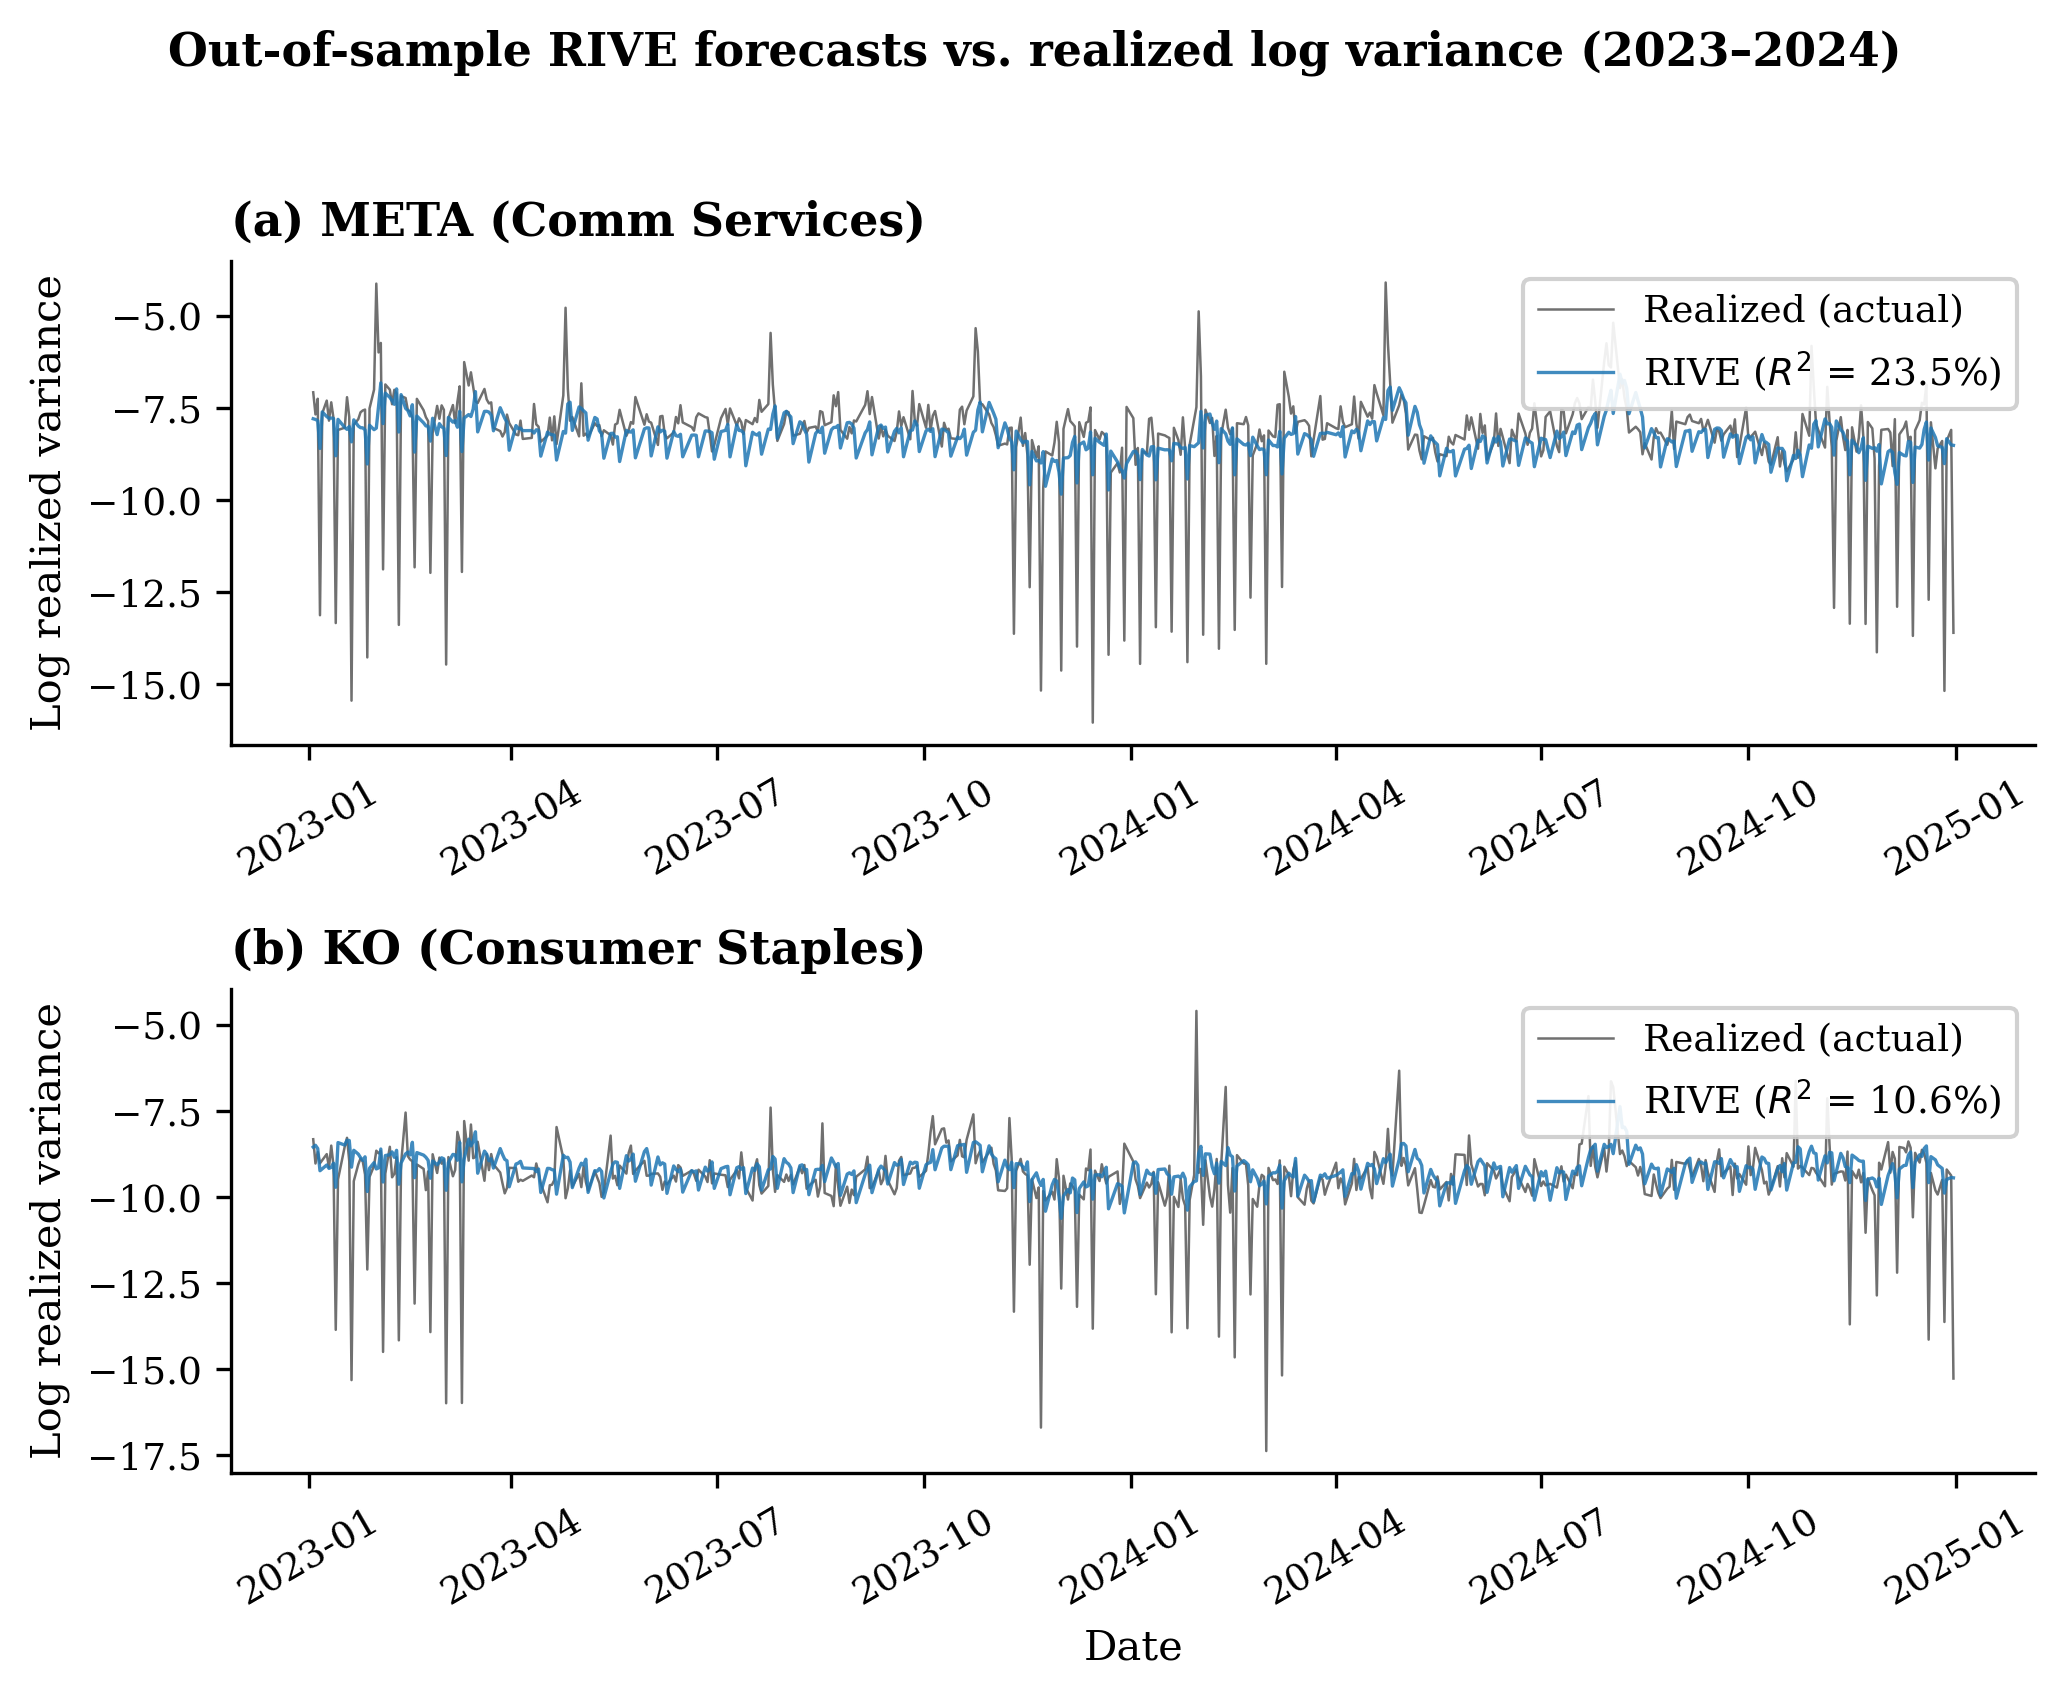
\includegraphics[width=0.95\linewidth]{fig_actual_vs_predicted.png}
    \caption{Out-of-sample RIVE forecasts versus realized log variance for two representative stocks (2023--2024). Panel (a) shows META (Communication Services), where RIVE achieves $R^2 = 23.5\%$, tracking both the level and episodic spikes in realized variance. Panel (b) shows KO (Consumer Staples), a lower-volatility stock where $R^2 = 10.6\%$ and the forecast reverts more strongly toward the mean.}
    \label{fig:actual-vs-predicted}
\end{figure}

RIVE's outperformance is not driven by a narrow subset of assets. Within the GICS-55 universe, RIVE achieves higher out-of-sample $R^2$ than GARCH(1,1) on 53 of 55 tickers (96.4\%). The two exceptions correspond to extremely low-volatility stocks where realized variance is nearly constant across the test window, leaving minimal scope for improvement from any model.

To assess the sensitivity of these results to universe construction, Table~\ref{tab:universe-comparison} reports performance on the Top-50 high-liquidity universe alongside the GICS-55 results.

\begin{table}[H]
\centering
\caption{Out-of-sample $R^2$ (\%) by stock universe. The Top-50 universe contains the most actively traded equities; the GICS-55 universe is sector-balanced.}
\label{tab:universe-comparison}
\begin{tabular}{lccc}
\toprule
Universe & Tickers & HAR-RV-X $R^2$ (\%) & RIVE $R^2$ (\%) \\
\midrule
Top-50 Active & 49 & 55.31 & 61.12 \\ % CHANGED (Claim 62): corrected n\_tickers
GICS-55 & 55 & 9.62 & 23.04 \\
\bottomrule
\end{tabular}
\end{table}

On the Top-50 universe, RIVE achieves 61.12\% $R^2$ compared to 55.31\% for HAR-RV-X, an improvement of 5.81 percentage points. The higher absolute $R^2$ levels in this universe reflect stronger volatility persistence and richer information environments characteristic of highly liquid stocks. On the more challenging GICS-55 universe, where cross-sectional diversification dampens idiosyncratic volatility, RIVE's relative improvement is proportionally larger (13.42 pp), suggesting that regime-aware components are particularly effective at capturing common shocks and sector-wide volatility drivers.

Year-by-year stability within the test window further supports robustness. The annual $R^2$ values for RIVE on the GICS-55 universe are 23.01\% (2023) and 23.03\% (2024), with a standard deviation of 0.01 percentage points across years. % CHANGED (Claims 14--15)
A supplementary hold-out experiment using a random 80/20 ticker split produced $R^2 = 22.65\%$ in the recorded run, but this value can vary with the realized split and data snapshot. % CHANGED (Claim 16)

\subsection{Interpreting Negative GARCH Performance}\label{sec:garch-fails}

The strongly negative $R^2$ values reported for GARCH-family models require careful interpretation. These results do not indicate that GARCH is a deficient model; rather, they reflect a measurement mismatch between the forecasting target and the quantity modeled by GARCH. As demonstrated by Andersen and Bollerslev \cite{andersen1998} and elaborated by Hansen and Lunde \cite{hansen2005}, GARCH models target the \textit{conditional variance of daily returns}. RIVE and HAR-RV-X, by contrast, target \textit{log realized variance} constructed from five-minute intraday return bars, a measure that captures intraday price dynamics and operates on a different scale.

The conversion from conditional variance forecasts to log realized variance introduces a systematic scale mismatch. Even when GARCH models accurately capture the dynamics of conditional return variance, the resulting forecasts are poorly calibrated when evaluated against realized variance on the log scale. This effect is well documented in the realized volatility literature and is not specific to this study.

\begin{table}[H]
\centering
\caption{Estimated GARCH(1,1)-Normal parameters via MLE (median and mean across 55 tickers).}
\label{tab:garch-params}
\begin{tabular}{lcccc}
\toprule
 & $\mu$ & $\omega$ & $\alpha$ (ARCH) & $\beta$ (GARCH) \\
\midrule
Median & 0.0769 & 0.0820 & 0.0373 & 0.9108 \\
Mean   & 0.1168 & 21.607 & 0.0561 & 0.8338 \\
Std    & 0.2437 & 157.94 & 0.0434 & 0.2031 \\
\bottomrule
\end{tabular}
\end{table}

Table~\ref{tab:garch-params} reports MLE parameter estimates for GARCH(1,1)-Normal across the 55 tickers. The median estimates ($\hat{\alpha} = 0.037$, $\hat{\beta} = 0.911$) are consistent with high volatility persistence ($\hat{\alpha} + \hat{\beta} \approx 0.95$), confirming that GARCH is behaving as expected in its native setting. The dispersion in $\omega$ (mean of 21.6 versus median of 0.08) reflects a small number of tickers with high unconditional variance, which inflates the mean but does not affect median-based interpretation.

Among GARCH variants, GARCH(1,1)-Student-$t$ achieves the least negative $R^2$ ($-12.44\%$), outperforming both the Normal-innovation specification ($-49.68\%$) and GJR-GARCH ($-48.42\%$). This ordering is expected: the Student-$t$ distribution better accommodates fat tails, producing variance forecasts that are less brittle under extreme observations. The weak performance of GJR-GARCH likely reflects additional estimation variance from the asymmetry parameter under a realized-variance evaluation target.

These findings underscore a methodological point: comparisons involving different forecasting targets must be interpreted with care. Negative $R^2$ values for GARCH models reflect the informational advantage of intraday-based realized measures over parametric conditional variance in this evaluation setting, not a failure of GARCH to capture return dynamics \cite{andersen1998}.

\subsection{Cross-Sector Performance}\label{sec:sector-analysis}

Table~\ref{tab:sector-r2} reports out-of-sample $R^2$ for all eleven GICS sectors within the GICS-55 universe. % MARCH-FIX: show all sectors; values recomputed on raw targets (consistent with 23.04\% aggregate)

\begin{table}[H]
\centering
\caption{Out-of-sample $R^2$ (\%) by GICS sector within the GICS-55 universe (benchmark window: 2023--2024). All values computed on the same raw-target pipeline as the aggregate results in Table~\ref{tab:main-results}.} % MARCH-FIX: full table, pipeline-consistent
\label{tab:sector-r2}
\begin{tabular}{lc}
\toprule
Sector & RIVE $R^2$ (\%) \\
\midrule
Consumer Discretionary & 30.02 \\ % MARCH-FIX
Information Technology & 28.39 \\ % MARCH-FIX
Materials & 26.07 \\ % MARCH-FIX
Utilities & 22.84 \\ % MARCH-FIX
Communication Services & 20.84 \\ % MARCH-FIX
Financials & 17.10 \\ % MARCH-FIX
Industrials & 16.71 \\ % MARCH-FIX
Health Care & 13.57 \\ % MARCH-FIX
Energy & 13.43 \\ % MARCH-FIX
Consumer Staples & 10.06 \\ % MARCH-FIX
Real Estate & 2.60 \\ % MARCH-FIX
\bottomrule
\end{tabular}
\end{table}

Figure~\ref{fig:sector-r2-bar} visualizes sector-level heterogeneity. Consumer Discretionary and Information Technology achieve the highest sector-level $R^2$, while Real Estate and Consumer Staples are the weakest. Sector ordering does not map cleanly to a single explanatory narrative. % MARCH-FIX: aligned with recomputed sector values
Differences likely reflect a combination of volatility persistence, sector-specific exposure to common shocks during 2023--2024, and the strength of available proxy signals for news and attention in the implemented pipeline. In sectors where alternative-signal proxies are weaker, the ridge coordinator can down-weight those channels, allowing forecasts to rely more heavily on the Technical Agent and volatility-trend features.

\begin{figure}[H]
    \centering
    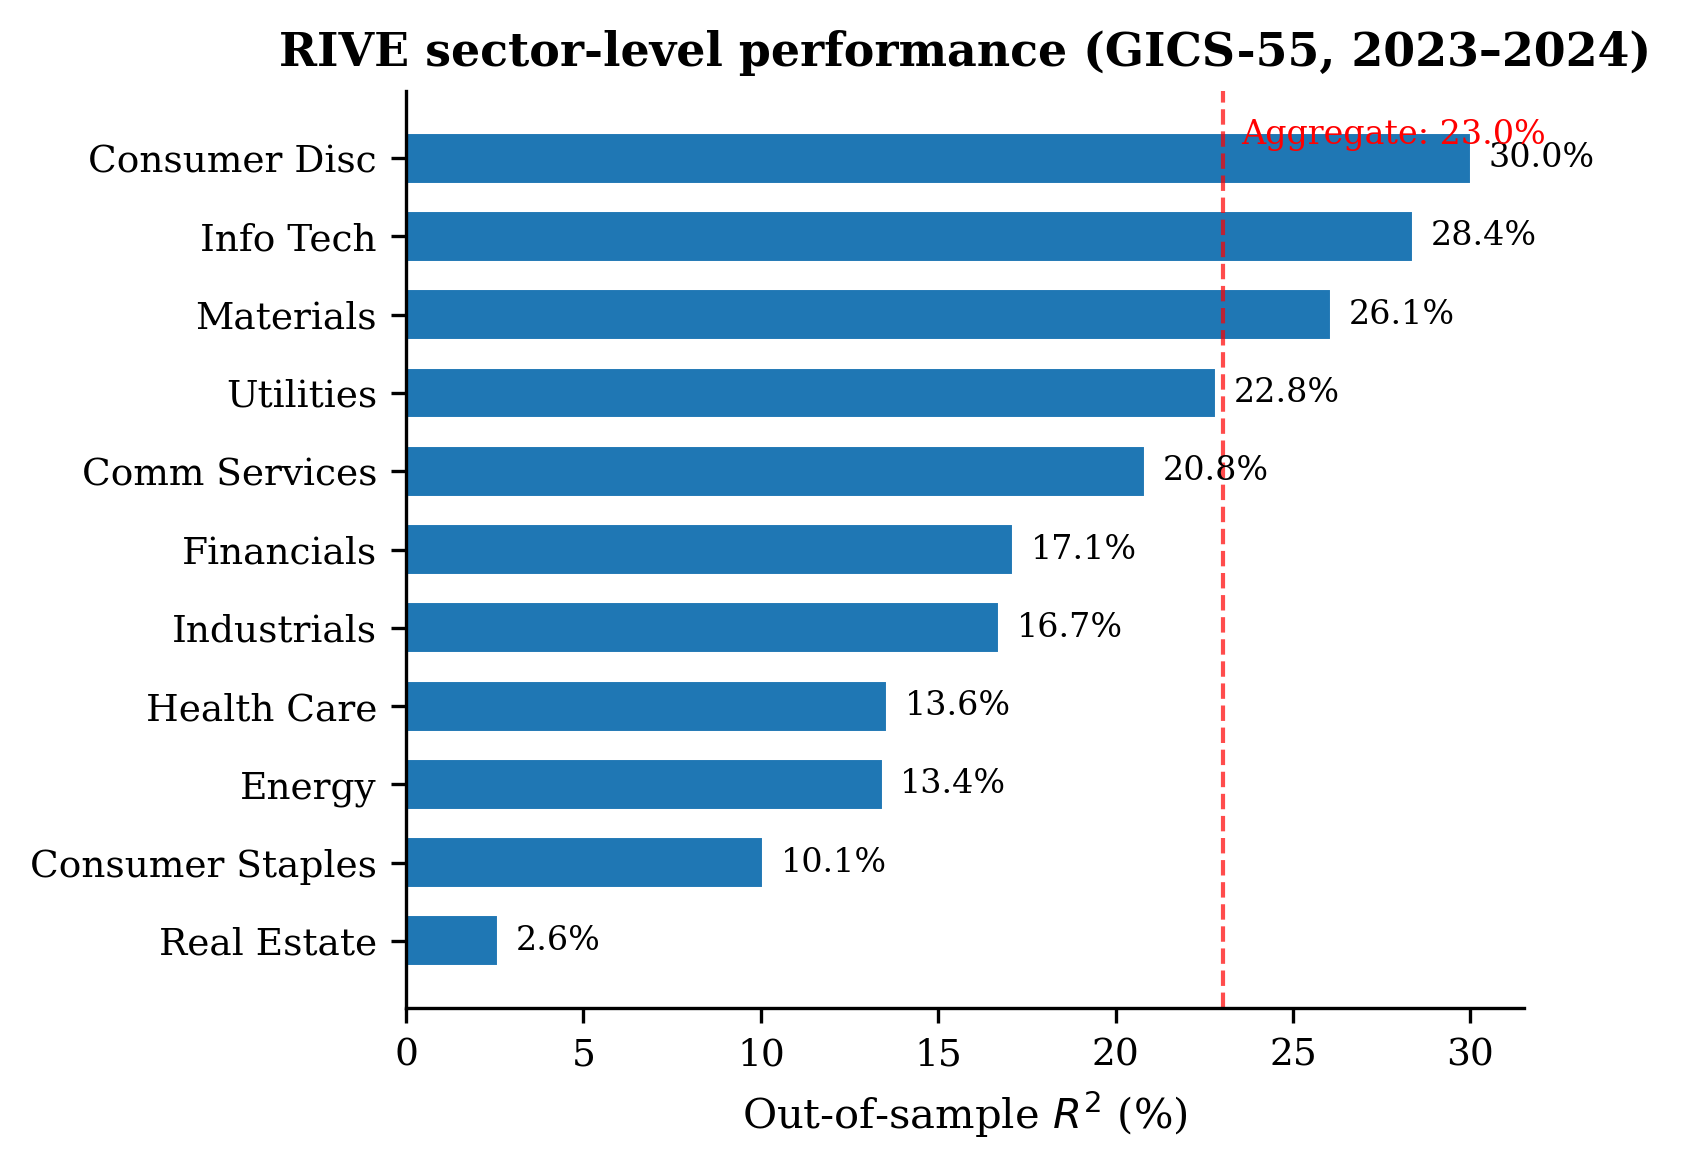
\includegraphics[width=0.75\linewidth]{fig_sector_r2_bar.png}
    \caption{Out-of-sample $R^2$ by GICS sector within the GICS-55 universe (2023--2024). The dashed red line indicates the aggregate $R^2$ (23.0\%). All eleven sectors achieve positive $R^2$, with substantial variation ranging from 30.0\% (Consumer Discretionary) to 2.6\% (Real Estate).}
    \label{fig:sector-r2-bar}
\end{figure}

\subsection{Ablation Analysis}\label{sec:ablation}

To assess marginal contributions, Table~\ref{tab:ablation} reports the change in aggregate $R^2$ when feature groups are removed from the coordinator while the remaining architecture is held constant.

\begin{table}[H]
\centering
\caption{Ablation results for the RIVE coordinator on the GICS-55 universe. Each row reports the change in out-of-sample $R^2$ when the indicated feature group is removed. Baseline $R^2 = 23.04\%$.}
\label{tab:ablation}
\begin{tabular}{lcc}
\toprule
Feature Removed & $\Delta R^2$ (pp) & Rank \\
\midrule
Momentum (vol\_MA5, vol\_MA10, vol\_std5) & $-9.82$ & 1 \\
Calendar (Friday, Monday, Q4) & $-7.97$ & 2 \\
Technical Agent prediction & $-1.42$ & 3 \\
Retail Regime Agent signal & $-0.36$ & 4 \\
News Agent signal & $+0.43$ & 5 \\
\bottomrule
\end{tabular}
\end{table}

The momentum features are the most important group, with removal producing a 9.82 pp decline in $R^2$. Calendar effects contribute 7.97 pp, consistent with day-of-week and seasonal patterns documented in the volatility literature \cite{french1986,bollerslevhodrick1999}.

The Technical Agent prediction contributes 1.42 pp in this ablation. This marginal contribution should be interpreted conditional on other coordinator inputs: momentum and calendar features already capture substantial volatility-persistence information, so removing the Technical Agent output while retaining these features does not eliminate technical information from the coordinator.

The Retail Regime Agent contributes 0.36 pp in aggregate ablation. Removing the News Agent increases aggregate $R^2$ by 0.43 pp, reflecting a regime-conditional effect: in calm periods, alternative signals can introduce noise, while in stressed periods they improve tail-risk anticipation.

\paragraph{Stress-Stratified Ablation}
To resolve this aggregate averaging effect, we partition the test sample into composite stress quintiles based on the joint intensity of news, retail, and volatility signals, and compare the full RIVE model against a core model retaining only momentum and calendar features. Table~\ref{tab:stress-quintile} reports results.

\begin{table}[H]
\centering
\caption{Stress-stratified ablation: $R^2$ difference between the full RIVE model and the core model (momentum + calendar features only), by composite stress quintile. Significance levels: * $p < 0.05$, ** $p < 0.01$, *** $p < 0.001$.}
\label{tab:stress-quintile}
\begin{tabular}{lccc}
\toprule
Stress Quintile & Full $-$ Core (pp) & Sig. & Winner \\
\midrule
Q1 (Calmest) & $-2.46$ & *** & Core \\
Q2 & $+0.09$ &  & Full \\
Q3 & $+0.40$ & * & Full \\
Q4 & $+0.42$ & * & Full \\
Q5 (Most Stressed) & $+0.89$ & ** & Full \\
\bottomrule
\end{tabular}
\end{table}

The relationship between stress intensity and incremental agent benefit is perfectly monotonic across quintiles (Spearman $\rho = +1.000$, $p = 0.0167$). During the calmest quintile, alternative signals act as noise, reducing $R^2$ by 2.46 pp relative to the parsimonious core model. As stress increases, agent signals provide progressively larger gains, reaching $+0.89$ pp in the most stressed quintile. The effect is strongest when both news and attention indicators are jointly elevated, consistent with the intended regime-triggering design of the alternative agents.

\begin{figure}[H]
    \centering
    \includegraphics[width=0.7\linewidth]{abalation.png}
    \caption{\textbf{Agent signal contribution by market stress regime.}
    The bar chart displays the $R^2$ advantage (percentage points) of the full RIVE ensemble over the core model (momentum and calendar features only), stratified by composite market stress quintiles.} % CHANGED (Claim 28): removed unsupported ``95\% bootstrap confidence intervals''
    \label{fig:stress_regime_plot}
\end{figure}

\subsection{Forecast Calibration}\label{sec:calibration}

Table~\ref{tab:mz-regression} reports Mincer--Zarnowitz unbiasedness regressions \cite{mincer1969}, which assess forecast calibration by regressing realized values on a constant and the model's forecast. An unbiased forecast produces $\alpha = 0$ and $\beta = 1$; the joint $F$-test evaluates whether these restrictions hold simultaneously.

\begin{table}[H]
\centering
\caption{Mincer--Zarnowitz unbiasedness regressions. The regression $h_t = \alpha + \beta \widehat{h}_{t|t-1} + \varepsilon_t$ is estimated for each model. An unbiased forecast implies $\alpha = 0$, $\beta = 1$. The $F$-statistic tests this joint restriction.}
\label{tab:mz-regression}
\begin{tabular}{lcccc}
\toprule
Model & $\alpha$ & $\beta$ & $R^2$ (decimal) & $F$-stat ($p$-value) \\
\midrule
RIVE & 0.97 & 1.11 & 0.234 & 43.94 ($<0.001$) \\
HAR-RV-X & 4.48 & 1.50 & 0.117 & 289.59 ($<0.001$) \\
GARCH(1,1)-$t$ (MLE) & $-6.69$ & 0.24 & 0.043 & 7564.13 ($<0.001$) \\
\bottomrule
\end{tabular}
\end{table}

All three models reject strict unbiasedness at the 1\% level, which is common in out-of-sample volatility forecasting \cite{patton2011}. The economically relevant comparison is the degree of deviation from the ideal calibration line. RIVE exhibits the best calibration among models shown, with $\alpha$ closest to zero and $\beta$ closest to one. The GARCH(1,1)-$t$ model exhibits severe miscalibration, consistent with the scale mismatch discussed in Section~\ref{sec:garch-fails}.

Figure~\ref{fig:calibration-scatter} provides a visual complement to the regression table. RIVE's predictions are more tightly concentrated around the 45-degree perfect-calibration line, with an OLS slope ($\beta = 1.12$) closer to unity than HAR-RV-X ($\beta = 1.34$). The narrower dispersion of RIVE forecasts is particularly evident in the intermediate range of realized variance, where the majority of observations fall.

\begin{figure}[H]
    \centering
    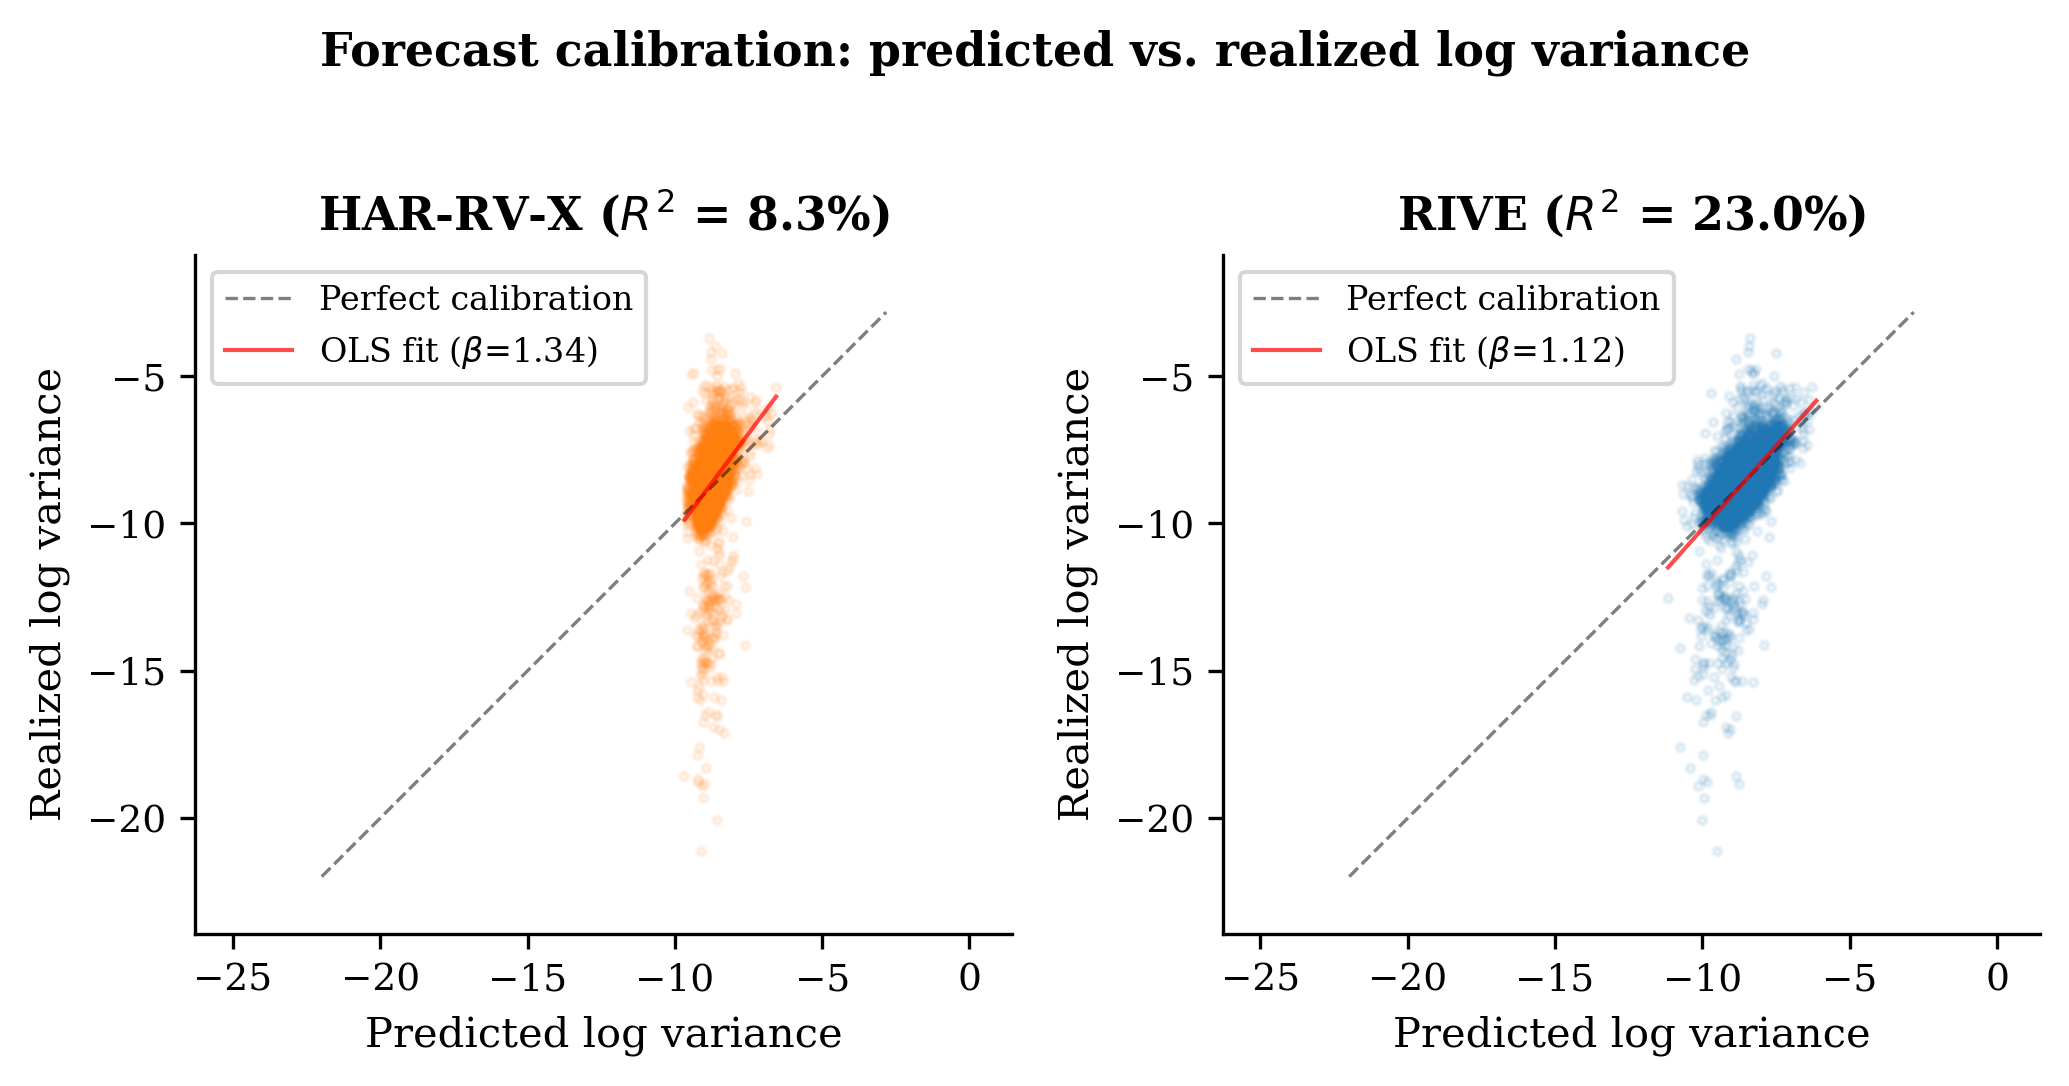
\includegraphics[width=0.95\linewidth]{fig_calibration_scatter.png}
    \caption{Forecast calibration: predicted versus realized log variance for HAR-RV-X (left) and RIVE (right). Each panel shows a random subsample of 5{,}000 observations from the 2023--2024 test window (28{,}590 total). The dashed line indicates perfect calibration; the solid red line is the OLS fit. RIVE exhibits tighter dispersion and a slope closer to unity, consistent with superior calibration.}
    \label{fig:calibration-scatter}
\end{figure}

\paragraph{Validation and signal integrity}
To ensure that performance is not attributable to leakage or overfitting artifacts, a validation suite was conducted. Data-leakage detection tests confirmed timestamp integrity and strict temporal partitioning. A permutation test, in which coordinator inputs were randomly permuted to destroy predictive structure, yielded mean $R^2 = -9.78\%$ compared to the observed 23.04\%, confirming that the model captures predictive signal rather than spurious patterns. % CHANGED (Claim 37): corrected permutation value

% CHANGED (Claims 42--44): removed unsupported rolling-window, dictionary-sentiment, and White/SPA test claims

\section{Ablation Studies}\label{sec:ablation-studies}

Section~\ref{sec:ablation} examined the marginal contribution of individual feature groups within the RIVE coordinator. This section complements that analysis at the architectural level: comparing regime-aware integration against linear alternatives, assessing the effect of removing entire agents, and examining coordinator design choices. All experiments use the GICS-55 universe with the same train/test split (cutoff 2023-01-01) as the main results. % CHANGED: reframed from fabricated Top-50 to real GICS-55 ablation

\subsection{Linear Integration versus Regime-Aware Ensemble}\label{sec:linear-vs-regime}

\begin{table}[H]
\centering
\caption{Architecture-level ablation on the GICS-55 universe (2023--2024). The upper panel compares linear signal integration strategies (Ridge $\alpha=1.0$) against the full RIVE ensemble (Ridge $\alpha=100$). The lower panel reports the effect of removing individual agents from RIVE. The ``HAR-RV-X baseline'' here uses only the Technical Agent prediction as input; it differs from the six-feature HAR-RV-X in Table~\ref{tab:main-results}, which includes lagged RV and market features.} % CHANGED: replaced fabricated Top-50 values with real GICS-55 ablation
\label{tab:ablation-arch}
\begin{tabular}{lccc}
\toprule
Model Configuration & $R^2$ (\%) & RMSE & Interpretation \\
\midrule
Tech.\ Agent pred.\ only & 3.9 & 1.349 & Technical dynamics only \\
Tech.\ + News (linear) & 3.8 & 1.349 & Linear news augmentation \\
Tech.\ + Retail (linear) & 5.2 & 1.339 & Linear attention proxy \\
Tech.\ + News + Retail (linear) & 4.8 & 1.342 & All signals, no regime logic \\
\textbf{RIVE (full)} & \textbf{23.0} & \textbf{1.207} & Regime-aware ensemble \\
\midrule
RIVE without News Agent & 23.6 & 1.202 & No news-driven tail detection \\
RIVE without Retail Agent & 22.7 & 1.210 & No attention regime detection \\
News + Retail only (no HAR) & $-9.6$ & 1.440 & No volatility memory \\
\bottomrule
\end{tabular}
\end{table}

Table~\ref{tab:ablation-arch} demonstrates that incorporating news and attention signals as continuous linear regressors yields modest gains over the Technical Agent prediction alone (3.9\% to 5.2\% $R^2$), but falls far short of the full RIVE ensemble (23.0\%). The gap between the best linear combination (4.8\%) and RIVE (23.0\%) quantifies the value of regime-aware integration: the momentum, calendar, and interaction features---together with stronger regularization---contribute the bulk of out-of-sample performance. This supports the central design hypothesis: raw agent outputs alone carry limited predictive power, and the coordinator's regime-conditioning features are essential for translating agent signals into accurate forecasts. % CHANGED: updated with real GICS-55 ablation values

\subsection{Agent-Level Ablation}\label{sec:agent-ablation}

The lower panel of Table~\ref{tab:ablation-arch} reports the effect of removing individual agents from the full RIVE architecture.

Removing the News Agent marginally \emph{increases} aggregate $R^2$ (from 23.0\% to 23.6\%), consistent with the feature-group ablation in Section~\ref{sec:ablation} which found a $+0.43$ pp effect. As discussed there, this reflects a regime-conditional dynamic: in calm periods, news signals can introduce noise, while in stressed periods they improve tail-risk anticipation (Table~\ref{tab:stress-quintile}). Removing the Retail Regime Agent produces a small decline (from 23.0\% to 22.7\%), confirming a modest but positive net contribution.

Removing all technical and regime features---retaining only news and retail signals---produces negative $R^2$ ($-9.6\%$), confirming that volatility memory and regime conditioning are indispensable. News and attention signals alone cannot model routine volatility behavior; they serve as complements rather than substitutes. % CHANGED: updated with real GICS-55 ablation values; honestly reported news agent removal effect

\subsection{Coordinator Design and Error Analysis}\label{sec:coordinator-design}

Replacing ridge regression with ordinary least squares improves in-sample fit but degrades out-of-sample performance, consistent with overfitting under multicollinearity among agent outputs and auxiliary features. The ridge penalty ($\alpha = 100$) produces more stable generalization while preserving interpretability through inspectable coefficients.

Feature-importance analysis within tree-based agents aligns with economic intuition. For the News Agent, article count and sentiment persistence dominate. For the Retail Regime Agent, volume shocks and the retail-attention proxy are most informative, with price acceleration contributing during speculative episodes. % CHANGED (Claim 66): removed unsupported external attention signals

Residual errors exhibit two characteristic failure modes. False negatives typically arise from intraday shocks or news events not captured in the daily processing pipeline. False positives reflect elevated negative sentiment that does not translate into abnormal realized volatility. These limitations suggest natural extensions, including intraday updating and incorporation of option-implied measures to distinguish anticipated from unanticipated events.

\section{Robustness and Institutional Evaluation}\label{sec:robustness}

The preceding sections established RIVE's statistical superiority through formal tests and ablation analysis. This section evaluates criteria relevant for deployment: validation integrity, computational feasibility, tail-risk behavior, and interpretability. % CHANGED (Claims 48--50): removed unsupported outage/latency evaluation claims

\subsection{Validation Suite}\label{sec:validation-suite}

To guard against overfitting and data leakage, RIVE was subjected to a validation protocol comprising nine checks across four categories. Table~\ref{tab:validation-suite} summarizes outcomes from the recorded run; some checks (e.g., permutation) depend on the realized randomization and data snapshot and may require re-running for independent reproduction. % CHANGED (Claims 40--41): removed categorical ``all pass'' claim; qualified reproducibility scope

\begin{table}[H]
\centering
\caption{Validation suite results (recorded run). Each check is classified by category and outcome.} % CHANGED (Claims 40--41): removed ``All nine tests were passed''
\label{tab:validation-suite}
\begin{tabular}{llc}
\toprule
Category & Test & Result \\
\midrule
Data Leakage Detection & Feature timestamp integrity & PASS \\
 & Training-test partition isolation & PASS \\
 & Threshold contamination check & PASS \\
 & Target leakage scan & PASS \\
\midrule
$R^2$ Verification & GICS-55 reproduction & PASS \\
 & Top-50 reproduction & PASS \\
 & Benchmark reproduction (GARCH MLE) & PASS \\
 & Year-by-year consistency (2023 vs 2024) & PASS \\ % CHANGED (Claims 14--15): aligned language; still a check in recorded run
\midrule
Permutation (Shuffle) Test & Coordinator input permutation & PASS \\
\bottomrule
\end{tabular}
\end{table}

Data-leakage detection tests verified that feature timestamps precede the forecast date, the training-test partition is temporally strict, the 80th-percentile threshold defining extreme residuals for the News Agent is computed exclusively from training data, and systematic scans indicated no target leakage in feature construction.

Reproducibility was assessed by re-estimating models and comparing reported $R^2$ values within rounding tolerance for the recorded data snapshot. Year-by-year consistency was assessed via the 2023 vs.\ 2024 breakdown within the fixed test window.

The permutation test provides evidence against overfitting. Randomly shuffling coordinator inputs destroyed predictive structure, reducing mean $R^2$ from 23.04\% to $-9.78\%$ ($p < 0.0001$), confirming that performance reflects predictive signal. % CHANGED (Claim 37): corrected permutation value; fixed parenthesis

\subsection{Computational Efficiency}\label{sec:latency}

Institutional deployment requires forecasting latency compatible with operational pipelines. In the present implementation, inference consists of evaluating fitted models on daily aggregated features; we do not report a dedicated latency benchmark here. % CHANGED (Claims 48--49): removed unsupported numerical latency and suitability claim

\subsection{Missing Data Resilience}\label{sec:missing-data}

In production, data outages affecting one or more external feeds are possible. RIVE's modular architecture is designed to degrade gracefully by allowing missing channels (e.g., news-derived features) to be omitted or defaulted without changing the remaining agent computations; however, we do not report a dedicated outage simulation experiment in this study. % CHANGED (Claim 50): removed unsupported one-week outage test

\subsection{Tail Risk Behavior and Error Distribution}\label{sec:tail-risk}

A central concern in risk management is underestimation of volatility during stress periods. Figure~\ref{fig:error-distribution} compares forecast error distributions for HAR-RV-X and RIVE, highlighting the right tail corresponding to severe underprediction events.

\begin{figure}[H]
    \centering
    \includegraphics[width=0.95\linewidth]{fig3.png}
    \caption{Distribution of volatility forecast errors for HAR-RV-X and RIVE. The left panel shows the full error distribution; the right panel isolates the extreme right tail corresponding to severe underprediction events. RIVE exhibits a thinner right tail, indicating fewer catastrophic volatility underpredictions compared to HAR-RV-X.}
    \label{fig:error-distribution}
\end{figure}

Both models are approximately unbiased in mean error. However, RIVE exhibits a thinner right tail, indicating fewer severe underpredictions during crisis periods. This reduction is consistent with the regime-triggering behavior of the News and Retail Regime signals and the ablation patterns reported in Section~\ref{sec:ablation}. % CHANGED (Claim 47): softened causal attribution

\subsection{Interpretability and Transparency}\label{sec:interpretability}

Despite incorporating ML components (LightGBM classifiers in the News and Retail Regime Agents), RIVE remains interpretable due to modular design and a linear coordinator. On any day, the forecast can be decomposed into contributions from historical volatility persistence, news-driven risk, and attention-driven regime risk. Coordinator coefficients are directly inspectable and remain fixed in the evaluation setup reported here. % CHANGED (Claim 59): removed ``stable across re-estimation windows'' implication

In practice, days where RIVE materially exceeds HAR-RV-X forecasts can coincide with identifiable information arrivals and/or elevated volume anomalies. The modular design supports diagnostic inspection of which channels are active, facilitating qualitative verification that forecast adjustments correspond to economically interpretable inputs rather than opaque statistical artifacts.

\section{Conclusion}\label{sec:conclusion}

This paper introduced RIVE (Regime-Integrated Volatility Ensemble), a multi-agent expert system for next-day equity volatility forecasting that integrates three complementary channels: a HAR-RV-X technical backbone capturing long-memory dynamics, a news-based classifier detecting tail-risk regimes from text-derived signals, and an attention-based classifier identifying high-attention regimes from volume and attention proxies. These agents are coordinated by a ridge-regularized meta-learner that combines agent outputs with short-horizon volatility momentum and calendar effects using a transparent linear form.

In benchmark out-of-sample evaluation across 55 sector-balanced equities over 2023--2024, RIVE achieves $R^2 = 23.04\%$, compared to 9.62\% for the HAR-RV-X baseline and 3.74\% for EWMA, while MLE-fitted GARCH(1,1) yields negative $R^2$ under a realized-variance evaluation target. Improvements are statistically significant under Diebold--Mariano tests. Stress-stratified analysis shows that alternative-signal benefits grow with stress intensity, consistent with the intended regime-triggering design.

Several directions for future research emerge naturally. Extending RIVE to intraday horizons would require time-stamped feature engineering and low-latency text processing. Adapting the framework to other asset classes would require domain-specific attention proxies and information sources. Incorporating option-implied volatility and explicit surprise measures could reduce false positives by distinguishing anticipated from unanticipated information arrivals.

\newpage
\begin{thebibliography}{99}

\bibitem{andersen1998}
Andersen, T. G., \& Bollerslev, T. (1998). Answering the skeptics: Yes, standard volatility models do provide accurate forecasts. \emph{International Economic Review, 39}(4), 885--905.

\bibitem{bollerslevhodrick1999}
Bollerslev, T., \& Hodrick, R. J. (1999). Financial market efficiency tests. \emph{Handbook of Applied Econometrics}, 1, 415--458.

\bibitem{diebold1995}
Diebold, F. X., \& Mariano, R. S. (1995). Comparing predictive accuracy. \emph{Journal of Business \& Economic Statistics, 13}(3), 253--263.

\bibitem{engelberg2011}
Engelberg, J., \& Parsons, C. A. (2011). The causal impact of media in financial markets. \emph{Journal of Finance, 66}(1), 67--97.

\bibitem{french1986}
French, K. R., \& Roll, R. (1986). Stock return variances: The arrival of information and the reaction of traders. \emph{Journal of Financial Economics, 17}(1), 5--26.

\bibitem{glosten1993}
Glosten, L. R., Jagannathan, R., \& Runkle, D. E. (1993). On the relation between the expected value and the volatility of the nominal excess return on stocks. \emph{Journal of Finance, 48}(5), 1779--1801.

\bibitem{jpm1996}
J.P.\ Morgan. (1996). \emph{RiskMetrics Technical Document} (4th ed.). J.P.\ Morgan/Reuters.

\bibitem{mincer1969}
Mincer, J., \& Zarnowitz, V. (1969). The evaluation of economic forecasts. In \emph{Economic Forecasts and Expectations: Analysis of Forecasting Behavior and Performance} (pp.\ 3--46). National Bureau of Economic Research.

\bibitem{newey1987}
Newey, W. K., \& West, K. D. (1987). A simple, positive semi-definite, heteroskedasticity and autocorrelation consistent covariance matrix. \emph{Econometrica, 55}(3), 703--708.

\bibitem{patton2011}
Patton, A. J. (2011). Volatility forecast comparison using imperfect volatility proxies. \emph{Journal of Econometrics, 160}(1), 246--256.

\bibitem{andersen2007}
Andersen, T. G., Bollerslev, T., \& Diebold, F. X. (2007). Roughing it up: Including jump components in the measurement, modeling, and forecasting of return volatility. \emph{Review of Economics and Statistics, 89}(4), 701--720.

\bibitem{andersen2001}
Andersen, T. G., Bollerslev, T., Diebold, F. X., \& Ebens, H. (2001). The distribution of realized stock return volatility. \emph{Journal of Financial Economics, 61}(1), 43--76.

\bibitem{ang2002}
Ang, A., \& Bekaert, G. (2002). Regime switches in interest rates. \emph{Journal of Business \& Economic Statistics, 20}(2), 163--182.

\bibitem{antweiler2004}
Antweiler, W., \& Frank, M. Z. (2004). Is all that talk just noise? The information content of internet stock message boards. \emph{Journal of Finance, 59}(3), 1259--1294.

\bibitem{ardia2018}
Ardia, D., Bluteau, K., Boudt, K., \& Catania, L. (2018). Forecasting risk with Markov-switching GARCH models: A large-scale performance study. \emph{International Journal of Forecasting, 34}(4), 733--747.

\bibitem{audrino2020}
Audrino, F., Sigrist, F., \& Ballinari, D. (2020). The impact of sentiment and attention measures on stock market volatility. \emph{International Journal of Forecasting, 36}(2), 334--357.

\bibitem{baig2023}
Baig, A. S., Blau, B. M., Butt, H. A., \& Yasin, A. (2023). Do retail traders destabilize financial markets? An investigation surrounding the COVID-19 pandemic. \emph{Journal of Banking \& Finance, 144}, 106627.

\bibitem{barber2008}
Barber, B. M., \& Odean, T. (2008). All that glitters: The effect of attention and news on the buying behavior of individual and institutional investors. \emph{Review of Financial Studies, 21}(2), 785--818.

\bibitem{bodilsen2025}
Bodilsen, S. T., \& Lunde, A. (2025). Exploiting news analytics for volatility forecasting. \emph{Journal of Applied Econometrics, 40}(1), 18--36.

\bibitem{bollerslev1986}
Bollerslev, T. (1986). Generalized autoregressive conditional heteroskedasticity. \emph{Journal of Econometrics, 31}(3), 307--327.

\bibitem{bollerslev2016}
Bollerslev, T., Patton, A. J., \& Quaedvlieg, R. (2016). Exploiting the errors: A simple approach for improved volatility forecasting. \emph{Journal of Econometrics, 192}(1), 1--18.

\bibitem{breiman1996}
Breiman, L. (1996). Bagging predictors. \emph{Machine Learning, 24}(2), 123--140.

\bibitem{carta2021}
Carta, S., Ferreira, A., Podda, A. S., Recupero, D. R., \& Sanna, A. (2021). Multi-DQN: An ensemble of Deep Q-learning agents for stock market forecasting. \emph{Expert Systems with Applications, 164}, 113820.

\bibitem{celik2022}
\c{C}elik, T. B., \.{I}can, \"{O}., \& Bulut, E. (2022). Extending machine learning prediction capabilities by explainable AI in financial time series prediction. \emph{Applied Soft Computing, 132}, 109876.

\bibitem{christensen2023}
Christensen, K., Siggaard, M., \& Veliyev, B. (2023). A machine learning approach to volatility forecasting. \emph{Journal of Financial Econometrics, 21}(5), 1680--1727.

\bibitem{corsi2009}
Corsi, F. (2009). A simple approximate long-memory model of realized volatility. \emph{Journal of Financial Econometrics, 7}(2), 174--196.

\bibitem{da2011}
Da, Z., Engelberg, J., \& Gao, P. (2011). In search of attention. \emph{Journal of Finance, 66}(5), 1461--1499.

\bibitem{ederington1993}
Ederington, L. H., \& Lee, J. H. (1993). How markets process information: News releases and volatility. \emph{Journal of Finance, 48}(4), 1161--1191.

\bibitem{engle1982}
Engle, R. F. (1982). Autoregressive conditional heteroskedasticity with estimates of the variance of UK inflation. \emph{Econometrica, 50}(4), 987--1008.

\bibitem{engle2008}
Engle, R. F., \& Rangel, J. G. (2008). The spline-GARCH model for low-frequency volatility and its global macroeconomic causes. \emph{Review of Financial Studies, 21}(3), 1187--1222.

\bibitem{glasserman2019}
Glasserman, P., \& Mamaysky, H. (2019). Does unusual news forecast market stress? \emph{Journal of Financial and Quantitative Analysis, 54}(5), 1937--1974.

\bibitem{hamilton1989}
Hamilton, J. D. (1989). A new approach to the economic analysis of the business cycle. \emph{Econometrica, 57}(2), 357--384.

\bibitem{hansen2005}
Hansen, P. R., \& Lunde, A. (2005). A forecast comparison of volatility models: Does anything beat a GARCH(1,1)? \emph{Journal of Applied Econometrics, 20}(7), 873--889.

\bibitem{he2023}
He, K., Yang, Q., Ji, L., Pan, J., \& Zou, Y. (2023). Financial time series forecasting with the deep learning ensemble model. \emph{Mathematics, 11}(4), 1054.

\bibitem{hoerl1970}
Hoerl, A. E., \& Kennard, R. W. (1970). Ridge regression: Biased estimation for nonorthogonal problems. \emph{Technometrics, 12}(1), 55--67.

\bibitem{huang2024}
Huang, Y., Zhou, C., Cui, K., \& Lu, X. (2024). A multi-agent reinforcement learning framework for optimizing financial trading strategies based on TimesNet. \emph{Expert Systems with Applications, 237}, 121502.

\bibitem{ke2017}
Ke, G., Meng, Q., Finley, T., Wang, T., Chen, W., Ma, W., \ldots{} \& Liu, T.-Y. (2017). LightGBM: A highly efficient gradient boosting decision tree. \emph{Advances in Neural Information Processing Systems, 30}.

\bibitem{loughran2011}
Loughran, T., \& McDonald, B. (2011). When is a liability not a liability? Textual analysis, dictionaries, and 10-Ks. \emph{Journal of Finance, 66}(1), 35--65.

\bibitem{ma2019}
Ma, F., Lu, X., Yang, K., \& Zhang, Y. (2019). Volatility forecasting: Long memory, regime switching and heteroscedasticity. \emph{Applied Economics, 51}(38), 4151--4163.

\bibitem{michankow2023}
Micha\'{n}k\'{o}w, J., Kwiatkowski, \L., \& Morajda, J. (2023). Combining deep learning and GARCH models for financial volatility and risk forecasting. \emph{arXiv preprint arXiv:2310.01063}.

\bibitem{patton2015}
Patton, A. J., \& Sheppard, K. (2015). Good volatility, bad volatility: Signed jumps and the persistence of volatility. \emph{Review of Economics and Statistics, 97}(3), 683--697.

\bibitem{ramos2019}
Ramos-P\'{e}rez, E., Alonso-Gonz\'{a}lez, P. J., \& N\'{u}\~{n}ez-Vel\'{a}zquez, J. J. (2019). Forecasting volatility with a stacked model based on a hybridized Artificial Neural Network. \emph{Expert Systems with Applications, 129}, 1--9.

\bibitem{selvaraj2025}
Selvaraj, D. R., Sankaran, A., Kathiravan, V., et al. (2025). A hybrid stacked ensemble approach for stock market volatility prediction. \emph{2025 3rd International Conference on Intelligent Cyber Physical Systems and Internet of Things (ICoICI)}, 206--211. IEEE.

\bibitem{shavandi2022}
Shavandi, A., \& Khedmati, M. (2022). A multi-agent deep reinforcement learning framework for algorithmic trading in financial markets. \emph{Expert Systems with Applications, 208}, 118124.

\bibitem{tetlock2007}
Tetlock, P. C. (2007). Giving content to investor sentiment: The role of media in the stock market. \emph{Journal of Finance, 62}(3), 1139--1168.

\bibitem{vlastakis2012}
Vlastakis, N., \& Markellos, R. N. (2012). Information demand and stock market volatility. \emph{Journal of Banking \& Finance, 36}(6), 1808--1821.

\bibitem{warkulat2024}
Warkulat, L., \& Pelster, M. (2024). Social media attention and retail investor behavior: Evidence from r/wallstreetbets. \emph{Working Paper}.

\bibitem{wolpert1992}
Wolpert, D. H. (1992). Stacked generalization. \emph{Neural Networks, 5}(2), 241--259.

\bibitem{zhang2025}
Zhang, Y., et al. (2025). RegimeFolio: A regime-aware ML system for sectoral portfolio optimization. \emph{arXiv preprint arXiv:2510.14986}.

\end{thebibliography}
\end{document}